\documentclass[twoside]{book}

% Packages required by doxygen
\usepackage{fixltx2e}
\usepackage{calc}
\usepackage{doxygen}
\usepackage[export]{adjustbox} % also loads graphicx
\usepackage{graphicx}
\usepackage[utf8]{inputenc}
\usepackage{makeidx}
\usepackage{multicol}
\usepackage{multirow}
\PassOptionsToPackage{warn}{textcomp}
\usepackage{textcomp}
\usepackage[nointegrals]{wasysym}
\usepackage[table]{xcolor}

% NLS support packages
\usepackage[spanish]{babel}
% Font selection
\usepackage[T1]{fontenc}
\usepackage[scaled=.90]{helvet}
\usepackage{courier}
\usepackage{amssymb}
\usepackage{sectsty}
\renewcommand{\familydefault}{\sfdefault}
\allsectionsfont{%
  \fontseries{bc}\selectfont%
  \color{darkgray}%
}
\renewcommand{\DoxyLabelFont}{%
  \fontseries{bc}\selectfont%
  \color{darkgray}%
}
\newcommand{\+}{\discretionary{\mbox{\scriptsize$\hookleftarrow$}}{}{}}

% Page & text layout
\usepackage{geometry}
\geometry{%
  a4paper,%
  top=2.5cm,%
  bottom=2.5cm,%
  left=2.5cm,%
  right=2.5cm%
}
\tolerance=750
\hfuzz=15pt
\hbadness=750
\setlength{\emergencystretch}{15pt}
\setlength{\parindent}{0cm}
\setlength{\parskip}{3ex plus 2ex minus 2ex}
\makeatletter
\renewcommand{\paragraph}{%
  \@startsection{paragraph}{4}{0ex}{-1.0ex}{1.0ex}{%
    \normalfont\normalsize\bfseries\SS@parafont%
  }%
}
\renewcommand{\subparagraph}{%
  \@startsection{subparagraph}{5}{0ex}{-1.0ex}{1.0ex}{%
    \normalfont\normalsize\bfseries\SS@subparafont%
  }%
}
\makeatother

% Headers & footers
\usepackage{fancyhdr}
\pagestyle{fancyplain}
\fancyhead[LE]{\fancyplain{}{\bfseries\thepage}}
\fancyhead[CE]{\fancyplain{}{}}
\fancyhead[RE]{\fancyplain{}{\bfseries\leftmark}}
\fancyhead[LO]{\fancyplain{}{\bfseries\rightmark}}
\fancyhead[CO]{\fancyplain{}{}}
\fancyhead[RO]{\fancyplain{}{\bfseries\thepage}}
\fancyfoot[LE]{\fancyplain{}{}}
\fancyfoot[CE]{\fancyplain{}{}}
\fancyfoot[RE]{\fancyplain{}{\bfseries\scriptsize Generado por Doxygen }}
\fancyfoot[LO]{\fancyplain{}{\bfseries\scriptsize Generado por Doxygen }}
\fancyfoot[CO]{\fancyplain{}{}}
\fancyfoot[RO]{\fancyplain{}{}}
\renewcommand{\footrulewidth}{0.4pt}
\renewcommand{\chaptermark}[1]{%
  \markboth{#1}{}%
}
\renewcommand{\sectionmark}[1]{%
  \markright{\thesection\ #1}%
}

% Indices & bibliography
\usepackage{natbib}
\usepackage[titles]{tocloft}
\setcounter{tocdepth}{3}
\setcounter{secnumdepth}{5}
\makeindex

% Hyperlinks (required, but should be loaded last)
\usepackage{ifpdf}
\ifpdf
  \usepackage[pdftex,pagebackref=true]{hyperref}
\else
  \usepackage[ps2pdf,pagebackref=true]{hyperref}
\fi
\hypersetup{%
  colorlinks=true,%
  linkcolor=blue,%
  citecolor=blue,%
  unicode%
}

% Custom commands
\newcommand{\clearemptydoublepage}{%
  \newpage{\pagestyle{empty}\cleardoublepage}%
}

\usepackage{caption}
\captionsetup{labelsep=space,justification=centering,font={bf},singlelinecheck=off,skip=4pt,position=top}

%===== C O N T E N T S =====

\begin{document}

% Titlepage & ToC
\hypersetup{pageanchor=false,
             bookmarksnumbered=true,
             pdfencoding=unicode
            }
\pagenumbering{alph}
\begin{titlepage}
\vspace*{7cm}
\begin{center}%
{\Large Paint }\\
\vspace*{1cm}
{\large Generado por Doxygen 1.8.13}\\
\end{center}
\end{titlepage}
\clearemptydoublepage
\pagenumbering{roman}
\tableofcontents
\clearemptydoublepage
\pagenumbering{arabic}
\hypersetup{pageanchor=true}

%--- Begin generated contents ---
\chapter{Página principal}
\label{index}\hypertarget{index}{}El codigo esta estructurado para que se use como la tortuga original de python. el algoritmo usa calculos matematicos basicos. 
\chapter{Indice jerárquico}
\section{Jerarquía de la clase}
Esta lista de herencias esta ordenada aproximadamente por orden alfabético\+:\begin{DoxyCompactList}
\item \contentsline{section}{Abstract\+Factory}{\pageref{classAbstractFactory}}{}
\begin{DoxyCompactList}
\item \contentsline{section}{paint1}{\pageref{classpaint1}}{}
\item \contentsline{section}{paint2}{\pageref{classpaint2}}{}
\end{DoxyCompactList}
\item \contentsline{section}{arbol}{\pageref{classarbol}}{}
\item \contentsline{section}{builder}{\pageref{classbuilder}}{}
\begin{DoxyCompactList}
\item \contentsline{section}{arbol\+\_\+normal}{\pageref{classarbol__normal}}{}
\end{DoxyCompactList}
\item \contentsline{section}{coordenada}{\pageref{structcoordenada}}{}
\item \contentsline{section}{director}{\pageref{classdirector}}{}
\item \contentsline{section}{flor}{\pageref{classflor}}{}
\begin{DoxyCompactList}
\item \contentsline{section}{flor\+\_\+bonita}{\pageref{classflor__bonita}}{}
\item \contentsline{section}{flor\+\_\+fea}{\pageref{classflor__fea}}{}
\item \contentsline{section}{flor\+\_\+regular}{\pageref{classflor__regular}}{}
\end{DoxyCompactList}
\item \contentsline{section}{hoja}{\pageref{classhoja}}{}
\item \contentsline{section}{nieve}{\pageref{classnieve}}{}
\item \contentsline{section}{particles}{\pageref{classparticles}}{}
\item \contentsline{section}{plano}{\pageref{classplano}}{}
\item \contentsline{section}{rama}{\pageref{classrama}}{}
\item \contentsline{section}{snow\+\_\+flyweight}{\pageref{classsnow__flyweight}}{}
\item \contentsline{section}{tronco}{\pageref{classtronco}}{}
\end{DoxyCompactList}

\chapter{Índice de clases}
\section{Lista de clases}
Lista de las clases, estructuras, uniones e interfaces con una breve descripción\+:\begin{DoxyCompactList}
\item\contentsline{section}{\hyperlink{classAbstractFactory}{Abstract\+Factory} \\*La clase \hyperlink{classAbstractFactory}{Abstract\+Factory} contiene funciones para crear todo el paint  Se instancia el dato miembro }{\pageref{classAbstractFactory}}{}
\item\contentsline{section}{\hyperlink{classarbol}{arbol} \\*La clase arbol contiene la funcion drawn para visualizar el arbol  Se instancia los datos miembros que son punteros a las partes del arbol }{\pageref{classarbol}}{}
\item\contentsline{section}{\hyperlink{classarbol__normal}{arbol\+\_\+normal} \\*La clase \hyperlink{classarbol__normal}{arbol\+\_\+normal} hereda del arbol, estes es un arbol normal y unico. Tambien puede ser modificado.  Las funciones apuntan a las clases de las partes del arbol, asi como tambien son void }{\pageref{classarbol__normal}}{}
\item\contentsline{section}{\hyperlink{classbuilder}{builder} \\*La clase builder contiene las funciones gettronco, gethojas, getramas para obtener las caracteristicas del arbol en sus clases hijas  Las funciones son virtual-\/puras y apuntan a las clases de las partes del arbol }{\pageref{classbuilder}}{}
\item\contentsline{section}{\hyperlink{structcoordenada}{coordenada} }{\pageref{structcoordenada}}{}
\item\contentsline{section}{\hyperlink{classdirector}{director} \\*La clase director es la que crea mediante el builder o mediante parametros }{\pageref{classdirector}}{}
\item\contentsline{section}{\hyperlink{classflor}{flor} \\*La clase flor contiene la funcion drawn para poder dibujarlo en pantalla  Se instancia el dato miembro }{\pageref{classflor}}{}
\item\contentsline{section}{\hyperlink{classflor__bonita}{flor\+\_\+bonita} \\*La clase \hyperlink{classflor__bonita}{flor\+\_\+bonita} es un tipo de flor en la que su dibujo es bonito,contiene la funcion drawn para poder visualizarlo, hereda de la clase flor  Se tiene constructor y destructor }{\pageref{classflor__bonita}}{}
\item\contentsline{section}{\hyperlink{classflor__fea}{flor\+\_\+fea} \\*La clase \hyperlink{classflor__fea}{flor\+\_\+fea} es un tipo de flor en la que su dibujo es feo,contiene la funcion drawn para poder visualizarlo, hereda de la clase flor  Se instancia el dato miembro }{\pageref{classflor__fea}}{}
\item\contentsline{section}{\hyperlink{classflor__regular}{flor\+\_\+regular} \\*La clase \hyperlink{classflor__regular}{flor\+\_\+regular} es un tipo de flor en la que su dibujo es \hyperlink{classflor__regular}{flor\+\_\+regular},contiene la funcion drawn para poder visualizarlo, hereda de la clase flor  Se instancia el dato miembro }{\pageref{classflor__regular}}{}
\item\contentsline{section}{\hyperlink{classhoja}{hoja} \\*La clase hoja contiene la funcion drawn para poder dibujará  Se instancia el dato miembro }{\pageref{classhoja}}{}
\item\contentsline{section}{\hyperlink{classnieve}{nieve} \\*La clase nieve es la clase que crea las particulas de nieve.  Se instancia el dato miembro }{\pageref{classnieve}}{}
\item\contentsline{section}{\hyperlink{classpaint1}{paint1} \\*La clase \hyperlink{classpaint1}{paint1} es un tipo de paint que tiene a arboles y a flores y tambien niev  Se instancia el dato miembro }{\pageref{classpaint1}}{}
\item\contentsline{section}{\hyperlink{classpaint2}{paint2} \\*La clase \hyperlink{classpaint2}{paint2} es un tipo de paint que tiene a arboles y a flores y tambien nieve  Se instancia el dato miembro }{\pageref{classpaint2}}{}
\item\contentsline{section}{\hyperlink{classparticles}{particles} \\*La clase particles es la calse que dibuja solo una particula.  Se instancia el dato miembro }{\pageref{classparticles}}{}
\item\contentsline{section}{\hyperlink{classplano}{plano} \\*La clase plano tiene los elementos basicos para empezar a dibujar como se hace en la python turtle.  Definicion de la funciones usadas en la clase }{\pageref{classplano}}{}
\item\contentsline{section}{\hyperlink{classrama}{rama} \\*La clase rama contiene la funcion drawn para poder dibujará.  Se instancia el dato miembro }{\pageref{classrama}}{}
\item\contentsline{section}{\hyperlink{classsnow__flyweight}{snow\+\_\+flyweight} \\*La clase \hyperlink{classsnow__flyweight}{snow\+\_\+flyweight} es el singleton que dibuja la nieve.  Se instancia el dato miembro }{\pageref{classsnow__flyweight}}{}
\item\contentsline{section}{\hyperlink{classtronco}{tronco} \\*La clase tronco contiene la funcion drawn para poder dibujarlo  Se instancia el dato miembro }{\pageref{classtronco}}{}
\end{DoxyCompactList}

\chapter{Indice de archivos}
\section{Lista de archivos}
Lista de todos los archivos documentados y con descripciones breves\+:\begin{DoxyCompactList}
\item\contentsline{section}{\hyperlink{Abstract_8cpp}{Abstract.\+cpp} \\*Implementacion de la clase paints para la creacion de paints en Glut Open\+GL }{\pageref{Abstract_8cpp}}{}
\item\contentsline{section}{\hyperlink{Abstract_8h}{Abstract.\+h} \\*Implementacion de la clase paints para la creacion de paints en Glut Open\+GL }{\pageref{Abstract_8h}}{}
\item\contentsline{section}{\hyperlink{builder__arbol_8cpp}{builder\+\_\+arbol.\+cpp} \\*Implementacion de la clase arbol para la creacion de arboles en Glut Open\+GL }{\pageref{builder__arbol_8cpp}}{}
\item\contentsline{section}{\hyperlink{builder__arbol_8h}{builder\+\_\+arbol.\+h} \\*Implementacion de la clase arbol para la creacion de arboles en Glut Open\+GL }{\pageref{builder__arbol_8h}}{}
\item\contentsline{section}{\hyperlink{factory__method__flor_8cpp}{factory\+\_\+method\+\_\+flor.\+cpp} \\*Implementacion de la clase flor para la creacion de flores en Glut Open\+GL }{\pageref{factory__method__flor_8cpp}}{}
\item\contentsline{section}{\hyperlink{factory__method__flor_8h}{factory\+\_\+method\+\_\+flor.\+h} \\*Implementacion de la clase flor para la creacion de flores en Glut Open\+GL }{\pageref{factory__method__flor_8h}}{}
\item\contentsline{section}{\hyperlink{flyweight__nieve_8cpp}{flyweight\+\_\+nieve.\+cpp} \\*Implementacion de la clase paints para la creacion de paints en Glut Open\+GL }{\pageref{flyweight__nieve_8cpp}}{}
\item\contentsline{section}{\hyperlink{flyweight__nieve_8h}{flyweight\+\_\+nieve.\+h} \\*Implementacion de la clase paints para la creacion de paints en Glut Open\+GL }{\pageref{flyweight__nieve_8h}}{}
\item\contentsline{section}{\hyperlink{plano_8cpp}{plano.\+cpp} \\*Implementacion de clase plano que permite hacer dibujos usando open\+GL }{\pageref{plano_8cpp}}{}
\item\contentsline{section}{\hyperlink{plano_8h}{plano.\+h} \\*Implementacion de clase plano que permite hacer dibujos usando open\+GL }{\pageref{plano_8h}}{}
\end{DoxyCompactList}

\chapter{Documentación de las clases}
\hypertarget{classAbstractFactory}{}\section{Referencia de la Clase Abstract\+Factory}
\label{classAbstractFactory}\index{Abstract\+Factory@{Abstract\+Factory}}


La clase \hyperlink{classAbstractFactory}{Abstract\+Factory} contiene funciones para crear todo el paint  Se instancia el dato miembro.  




{\ttfamily \#include $<$Abstract.\+h$>$}



Diagrama de herencias de Abstract\+Factory
\nopagebreak
\begin{figure}[H]
\begin{center}
\leavevmode
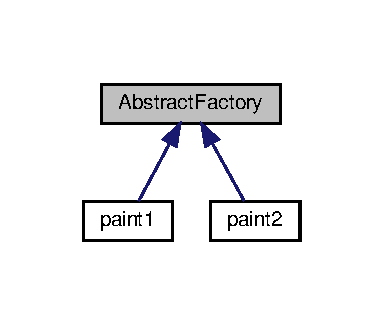
\includegraphics[width=184pt]{classAbstractFactory__inherit__graph}
\end{center}
\end{figure}
\subsection*{Métodos públicos}
\begin{DoxyCompactItemize}
\item 
\mbox{\Hypertarget{classAbstractFactory_a4a73c25633077f5c49681eb38cfaa42d}\label{classAbstractFactory_a4a73c25633077f5c49681eb38cfaa42d}} 
virtual \hyperlink{classarbol}{arbol} $\ast$ {\bfseries getarbol} ()=0
\item 
\mbox{\Hypertarget{classAbstractFactory_ac2e2c8c904de4282f1d49fe1231e441c}\label{classAbstractFactory_ac2e2c8c904de4282f1d49fe1231e441c}} 
virtual \hyperlink{classflor}{flor} $\ast$ {\bfseries get\+Flor} ()=0
\item 
\mbox{\Hypertarget{classAbstractFactory_a37a36d0033a932766221222cd981b157}\label{classAbstractFactory_a37a36d0033a932766221222cd981b157}} 
virtual \hyperlink{classnieve}{nieve} $\ast$ {\bfseries getnieve} ()=0
\end{DoxyCompactItemize}


\subsection{Descripción detallada}
La clase \hyperlink{classAbstractFactory}{Abstract\+Factory} contiene funciones para crear todo el paint  Se instancia el dato miembro. 

La documentación para esta clase fue generada a partir del siguiente fichero\+:\begin{DoxyCompactItemize}
\item 
\hyperlink{Abstract_8h}{Abstract.\+h}\end{DoxyCompactItemize}

\hypertarget{classarbol}{}\section{Referencia de la Clase arbol}
\label{classarbol}\index{arbol@{arbol}}


La clase arbol contiene la funcion drawn para visualizar el arbol  Se instancia los datos miembros que son punteros a las partes del arbol.  




{\ttfamily \#include $<$builder\+\_\+arbol.\+h$>$}



Diagrama de colaboración para arbol\+:
\nopagebreak
\begin{figure}[H]
\begin{center}
\leavevmode
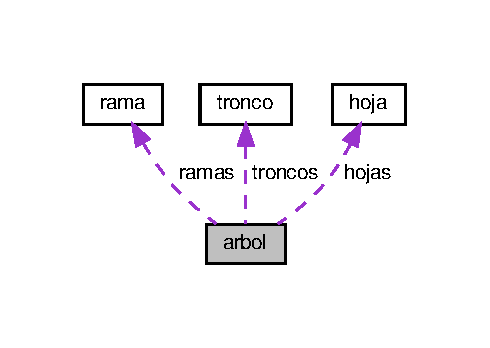
\includegraphics[width=235pt]{classarbol__coll__graph}
\end{center}
\end{figure}
\subsection*{Métodos públicos}
\begin{DoxyCompactItemize}
\item 
void \hyperlink{classarbol_a2b280a669a809d02bb86754349d7c339}{drawn} (\hyperlink{classplano}{plano} p, int x, int y)
\end{DoxyCompactItemize}
\subsection*{Atributos públicos}
\begin{DoxyCompactItemize}
\item 
\mbox{\Hypertarget{classarbol_a7e70557693f5d2ce7acc8071b2e3456f}\label{classarbol_a7e70557693f5d2ce7acc8071b2e3456f}} 
\hyperlink{classtronco}{tronco} $\ast$ {\bfseries troncos}
\item 
\mbox{\Hypertarget{classarbol_a6ace1361b0755b05450406a1495b947f}\label{classarbol_a6ace1361b0755b05450406a1495b947f}} 
\hyperlink{classhoja}{hoja} $\ast$ {\bfseries hojas}
\item 
\mbox{\Hypertarget{classarbol_ad98638d8955eb676de30474789fdbdd4}\label{classarbol_ad98638d8955eb676de30474789fdbdd4}} 
\hyperlink{classrama}{rama} $\ast$ {\bfseries ramas}
\end{DoxyCompactItemize}


\subsection{Descripción detallada}
La clase arbol contiene la funcion drawn para visualizar el arbol  Se instancia los datos miembros que son punteros a las partes del arbol. 

\subsection{Documentación de las funciones miembro}
\mbox{\Hypertarget{classarbol_a2b280a669a809d02bb86754349d7c339}\label{classarbol_a2b280a669a809d02bb86754349d7c339}} 
\index{arbol@{arbol}!drawn@{drawn}}
\index{drawn@{drawn}!arbol@{arbol}}
\subsubsection{\texorpdfstring{drawn()}{drawn()}}
{\footnotesize\ttfamily void arbol\+::drawn (\begin{DoxyParamCaption}\item[{\hyperlink{classplano}{plano}}]{p,  }\item[{int}]{x,  }\item[{int}]{y }\end{DoxyParamCaption})}

La funcion drawn recibe el plano y las coordenadas donde se dibujará. 
\begin{DoxyParams}{Parámetros}
{\em p,nos} & permite hacer uso de la tortuga. \\
\hline
{\em x} & es la coordenada x en la que se dibujará. \\
\hline
{\em y} & es la coordenada y en la que se dibujará. \\
\hline
\end{DoxyParams}


La documentación para esta clase fue generada a partir de los siguientes ficheros\+:\begin{DoxyCompactItemize}
\item 
\hyperlink{builder__arbol_8h}{builder\+\_\+arbol.\+h}\item 
\hyperlink{builder__arbol_8cpp}{builder\+\_\+arbol.\+cpp}\end{DoxyCompactItemize}

\hypertarget{classarbol__normal}{}\section{Referencia de la Clase arbol\+\_\+normal}
\label{classarbol__normal}\index{arbol\+\_\+normal@{arbol\+\_\+normal}}


La clase \hyperlink{classarbol__normal}{arbol\+\_\+normal} hereda del arbol, estes es un arbol normal y unico. Tambien puede ser modificado.  Las funciones apuntan a las clases de las partes del arbol, asi como tambien son void.  




{\ttfamily \#include $<$builder\+\_\+arbol.\+h$>$}



Diagrama de herencias de arbol\+\_\+normal
\nopagebreak
\begin{figure}[H]
\begin{center}
\leavevmode
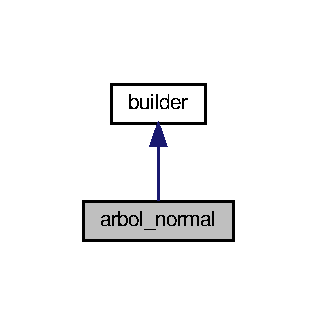
\includegraphics[width=152pt]{classarbol__normal__inherit__graph}
\end{center}
\end{figure}


Diagrama de colaboración para arbol\+\_\+normal\+:
\nopagebreak
\begin{figure}[H]
\begin{center}
\leavevmode
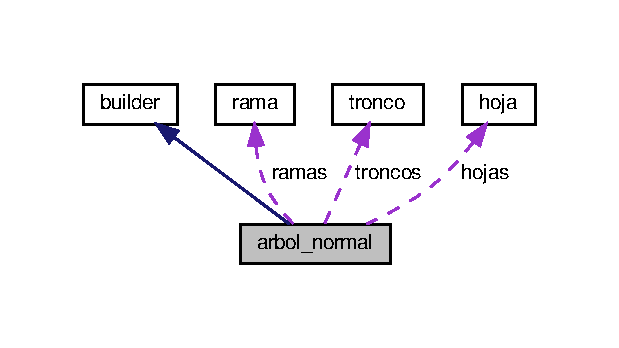
\includegraphics[width=297pt]{classarbol__normal__coll__graph}
\end{center}
\end{figure}
\subsection*{Métodos públicos}
\begin{DoxyCompactItemize}
\item 
void \hyperlink{classarbol__normal_a6f761bf112224d0478b63935a591d91c}{settronco} (int size)
\item 
void \hyperlink{classarbol__normal_a21fb8efde2259a78b694a81ecb543a07}{sethojas} (int size)
\item 
void \hyperlink{classarbol__normal_a48dbb830f192cf75d87adb80ec23ea7d}{setramas} (int size)
\item 
\hyperlink{classtronco}{tronco} $\ast$ \hyperlink{classarbol__normal_a24fdce164b50a74414b6a3d5ad4e99f6}{gettronco} ()
\item 
\hyperlink{classhoja}{hoja} $\ast$ \hyperlink{classarbol__normal_a999f324b73ff973d4b5b49e2403c637b}{gethojas} ()
\item 
\hyperlink{classrama}{rama} $\ast$ \hyperlink{classarbol__normal_a34c202fa845954e82719d3e86a5a0d9e}{getramas} ()
\end{DoxyCompactItemize}
\subsection*{Atributos públicos}
\begin{DoxyCompactItemize}
\item 
\mbox{\Hypertarget{classarbol__normal_adcb741c6f4ed4ec3d6fb5a2b3df936ca}\label{classarbol__normal_adcb741c6f4ed4ec3d6fb5a2b3df936ca}} 
\hyperlink{classtronco}{tronco} $\ast$ {\bfseries troncos}
\item 
\mbox{\Hypertarget{classarbol__normal_a4f210ae92daf183b8f703600853827aa}\label{classarbol__normal_a4f210ae92daf183b8f703600853827aa}} 
\hyperlink{classhoja}{hoja} $\ast$ {\bfseries hojas}
\item 
\mbox{\Hypertarget{classarbol__normal_a238920cdedd1261bcc372cd9b68e8086}\label{classarbol__normal_a238920cdedd1261bcc372cd9b68e8086}} 
\hyperlink{classrama}{rama} $\ast$ {\bfseries ramas}
\end{DoxyCompactItemize}


\subsection{Descripción detallada}
La clase \hyperlink{classarbol__normal}{arbol\+\_\+normal} hereda del arbol, estes es un arbol normal y unico. Tambien puede ser modificado.  Las funciones apuntan a las clases de las partes del arbol, asi como tambien son void. 

\subsection{Documentación de las funciones miembro}
\mbox{\Hypertarget{classarbol__normal_a999f324b73ff973d4b5b49e2403c637b}\label{classarbol__normal_a999f324b73ff973d4b5b49e2403c637b}} 
\index{arbol\+\_\+normal@{arbol\+\_\+normal}!gethojas@{gethojas}}
\index{gethojas@{gethojas}!arbol\+\_\+normal@{arbol\+\_\+normal}}
\subsubsection{\texorpdfstring{gethojas()}{gethojas()}}
{\footnotesize\ttfamily \hyperlink{classhoja}{hoja} $\ast$ arbol\+\_\+normal\+::gethojas (\begin{DoxyParamCaption}{ }\end{DoxyParamCaption})\hspace{0.3cm}{\ttfamily [virtual]}}

La funcion gethojas es un puntero a tronco, nos permite obtener las caracteristicas de este. 

Implementa \hyperlink{classbuilder_a03de42e8ec33a22c3635a6e946061b70}{builder}.

\mbox{\Hypertarget{classarbol__normal_a34c202fa845954e82719d3e86a5a0d9e}\label{classarbol__normal_a34c202fa845954e82719d3e86a5a0d9e}} 
\index{arbol\+\_\+normal@{arbol\+\_\+normal}!getramas@{getramas}}
\index{getramas@{getramas}!arbol\+\_\+normal@{arbol\+\_\+normal}}
\subsubsection{\texorpdfstring{getramas()}{getramas()}}
{\footnotesize\ttfamily \hyperlink{classrama}{rama} $\ast$ arbol\+\_\+normal\+::getramas (\begin{DoxyParamCaption}{ }\end{DoxyParamCaption})\hspace{0.3cm}{\ttfamily [virtual]}}

La funcion getramas es un puntero a tronco, nos permite obtener las caracteristicas de este. 

Implementa \hyperlink{classbuilder_a7b811cc1a2cffe9f3601faab0d85627b}{builder}.

\mbox{\Hypertarget{classarbol__normal_a24fdce164b50a74414b6a3d5ad4e99f6}\label{classarbol__normal_a24fdce164b50a74414b6a3d5ad4e99f6}} 
\index{arbol\+\_\+normal@{arbol\+\_\+normal}!gettronco@{gettronco}}
\index{gettronco@{gettronco}!arbol\+\_\+normal@{arbol\+\_\+normal}}
\subsubsection{\texorpdfstring{gettronco()}{gettronco()}}
{\footnotesize\ttfamily \hyperlink{classtronco}{tronco} $\ast$ arbol\+\_\+normal\+::gettronco (\begin{DoxyParamCaption}{ }\end{DoxyParamCaption})\hspace{0.3cm}{\ttfamily [virtual]}}

La funcion gettronco es un puntero a tronco, nos permite obtener las caracteristicas de este. 

Implementa \hyperlink{classbuilder_af81e62bdfc53bbdad5f1d8edc4b46ecd}{builder}.

\mbox{\Hypertarget{classarbol__normal_a21fb8efde2259a78b694a81ecb543a07}\label{classarbol__normal_a21fb8efde2259a78b694a81ecb543a07}} 
\index{arbol\+\_\+normal@{arbol\+\_\+normal}!sethojas@{sethojas}}
\index{sethojas@{sethojas}!arbol\+\_\+normal@{arbol\+\_\+normal}}
\subsubsection{\texorpdfstring{sethojas()}{sethojas()}}
{\footnotesize\ttfamily void arbol\+\_\+normal\+::sethojas (\begin{DoxyParamCaption}\item[{int}]{size }\end{DoxyParamCaption})}

La funcion sethojas recibe el tamano. 
\begin{DoxyParams}{Parámetros}
{\em size,nos} & permite definir el tamano pedido. \\
\hline
\end{DoxyParams}
\mbox{\Hypertarget{classarbol__normal_a48dbb830f192cf75d87adb80ec23ea7d}\label{classarbol__normal_a48dbb830f192cf75d87adb80ec23ea7d}} 
\index{arbol\+\_\+normal@{arbol\+\_\+normal}!setramas@{setramas}}
\index{setramas@{setramas}!arbol\+\_\+normal@{arbol\+\_\+normal}}
\subsubsection{\texorpdfstring{setramas()}{setramas()}}
{\footnotesize\ttfamily void arbol\+\_\+normal\+::setramas (\begin{DoxyParamCaption}\item[{int}]{size }\end{DoxyParamCaption})}

La funcion setramas recibe el tamano. 
\begin{DoxyParams}{Parámetros}
{\em size,nos} & permite definir el tamano pedido. \\
\hline
\end{DoxyParams}
\mbox{\Hypertarget{classarbol__normal_a6f761bf112224d0478b63935a591d91c}\label{classarbol__normal_a6f761bf112224d0478b63935a591d91c}} 
\index{arbol\+\_\+normal@{arbol\+\_\+normal}!settronco@{settronco}}
\index{settronco@{settronco}!arbol\+\_\+normal@{arbol\+\_\+normal}}
\subsubsection{\texorpdfstring{settronco()}{settronco()}}
{\footnotesize\ttfamily void arbol\+\_\+normal\+::settronco (\begin{DoxyParamCaption}\item[{int}]{size }\end{DoxyParamCaption})}

La funcion settronco recibe el tamano. 
\begin{DoxyParams}{Parámetros}
{\em size,nos} & permite definir el tamano pedido. \\
\hline
\end{DoxyParams}


La documentación para esta clase fue generada a partir de los siguientes ficheros\+:\begin{DoxyCompactItemize}
\item 
\hyperlink{builder__arbol_8h}{builder\+\_\+arbol.\+h}\item 
\hyperlink{builder__arbol_8cpp}{builder\+\_\+arbol.\+cpp}\end{DoxyCompactItemize}

\hypertarget{classbuilder}{}\section{Referencia de la Clase builder}
\label{classbuilder}\index{builder@{builder}}


La clase builder contiene las funciones gettronco, gethojas, getramas para obtener las caracteristicas del arbol en sus clases hijas  Las funciones son virtual-\/puras y apuntan a las clases de las partes del arbol.  




{\ttfamily \#include $<$builder\+\_\+arbol.\+h$>$}



Diagrama de herencias de builder
\nopagebreak
\begin{figure}[H]
\begin{center}
\leavevmode
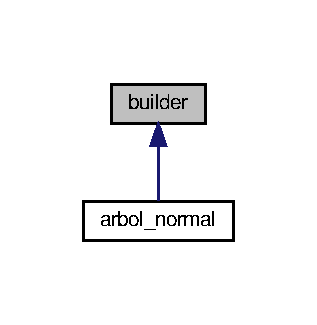
\includegraphics[width=152pt]{classbuilder__inherit__graph}
\end{center}
\end{figure}
\subsection*{Métodos públicos}
\begin{DoxyCompactItemize}
\item 
virtual \hyperlink{classtronco}{tronco} $\ast$ \hyperlink{classbuilder_af81e62bdfc53bbdad5f1d8edc4b46ecd}{gettronco} ()=0
\item 
virtual \hyperlink{classhoja}{hoja} $\ast$ \hyperlink{classbuilder_a03de42e8ec33a22c3635a6e946061b70}{gethojas} ()=0
\item 
virtual \hyperlink{classrama}{rama} $\ast$ \hyperlink{classbuilder_a7b811cc1a2cffe9f3601faab0d85627b}{getramas} ()=0
\end{DoxyCompactItemize}


\subsection{Descripción detallada}
La clase builder contiene las funciones gettronco, gethojas, getramas para obtener las caracteristicas del arbol en sus clases hijas  Las funciones son virtual-\/puras y apuntan a las clases de las partes del arbol. 

\subsection{Documentación de las funciones miembro}
\mbox{\Hypertarget{classbuilder_a03de42e8ec33a22c3635a6e946061b70}\label{classbuilder_a03de42e8ec33a22c3635a6e946061b70}} 
\index{builder@{builder}!gethojas@{gethojas}}
\index{gethojas@{gethojas}!builder@{builder}}
\subsubsection{\texorpdfstring{gethojas()}{gethojas()}}
{\footnotesize\ttfamily virtual \hyperlink{classhoja}{hoja}$\ast$ builder\+::gethojas (\begin{DoxyParamCaption}{ }\end{DoxyParamCaption})\hspace{0.3cm}{\ttfamily [pure virtual]}}

La funcion gethojas es virtual pura para que pueda ser heredada, utilizada y sobrescrita por las demas clases. 

Implementado en \hyperlink{classarbol__normal_a999f324b73ff973d4b5b49e2403c637b}{arbol\+\_\+normal}.

\mbox{\Hypertarget{classbuilder_a7b811cc1a2cffe9f3601faab0d85627b}\label{classbuilder_a7b811cc1a2cffe9f3601faab0d85627b}} 
\index{builder@{builder}!getramas@{getramas}}
\index{getramas@{getramas}!builder@{builder}}
\subsubsection{\texorpdfstring{getramas()}{getramas()}}
{\footnotesize\ttfamily virtual \hyperlink{classrama}{rama}$\ast$ builder\+::getramas (\begin{DoxyParamCaption}{ }\end{DoxyParamCaption})\hspace{0.3cm}{\ttfamily [pure virtual]}}

La funcion getramas es virtual pura para que pueda ser heredada, utilizada y sobrescrita por las demas clases. 

Implementado en \hyperlink{classarbol__normal_a34c202fa845954e82719d3e86a5a0d9e}{arbol\+\_\+normal}.

\mbox{\Hypertarget{classbuilder_af81e62bdfc53bbdad5f1d8edc4b46ecd}\label{classbuilder_af81e62bdfc53bbdad5f1d8edc4b46ecd}} 
\index{builder@{builder}!gettronco@{gettronco}}
\index{gettronco@{gettronco}!builder@{builder}}
\subsubsection{\texorpdfstring{gettronco()}{gettronco()}}
{\footnotesize\ttfamily virtual \hyperlink{classtronco}{tronco}$\ast$ builder\+::gettronco (\begin{DoxyParamCaption}{ }\end{DoxyParamCaption})\hspace{0.3cm}{\ttfamily [pure virtual]}}

La funcion gettronco es virtual pura para que pueda ser heredada, utilizada y sobrescrita por las demas clases. 

Implementado en \hyperlink{classarbol__normal_a24fdce164b50a74414b6a3d5ad4e99f6}{arbol\+\_\+normal}.



La documentación para esta clase fue generada a partir del siguiente fichero\+:\begin{DoxyCompactItemize}
\item 
\hyperlink{builder__arbol_8h}{builder\+\_\+arbol.\+h}\end{DoxyCompactItemize}

\hypertarget{structcoordenada}{}\section{Referencia de la Estructura coordenada}
\label{structcoordenada}\index{coordenada@{coordenada}}
\subsection*{Atributos públicos}
\begin{DoxyCompactItemize}
\item 
\mbox{\Hypertarget{structcoordenada_a58f4bd357e0e907cc46bcd35f5271e8e}\label{structcoordenada_a58f4bd357e0e907cc46bcd35f5271e8e}} 
t\+\_\+coord {\bfseries x}
\item 
\mbox{\Hypertarget{structcoordenada_a0048d987a8afd0cf94b8ec4a155fcad5}\label{structcoordenada_a0048d987a8afd0cf94b8ec4a155fcad5}} 
t\+\_\+coord {\bfseries y}
\item 
\mbox{\Hypertarget{structcoordenada_a379001d7331a9ecd1b85521e6c1162d3}\label{structcoordenada_a379001d7331a9ecd1b85521e6c1162d3}} 
int {\bfseries R}
\item 
\mbox{\Hypertarget{structcoordenada_a69897a5bd2f9713376d0dc541fd96de2}\label{structcoordenada_a69897a5bd2f9713376d0dc541fd96de2}} 
int {\bfseries G}
\item 
\mbox{\Hypertarget{structcoordenada_ad39661406d2665ff1efe3c695e81a933}\label{structcoordenada_ad39661406d2665ff1efe3c695e81a933}} 
int {\bfseries B}
\item 
\mbox{\Hypertarget{structcoordenada_a35322c013bfbef19997d61111767446f}\label{structcoordenada_a35322c013bfbef19997d61111767446f}} 
t\+\_\+coord {\bfseries grados}
\end{DoxyCompactItemize}


La documentación para esta estructura fue generada a partir del siguiente fichero\+:\begin{DoxyCompactItemize}
\item 
\hyperlink{plano_8h}{plano.\+h}\end{DoxyCompactItemize}

\hypertarget{classdirector}{}\section{Referencia de la Clase director}
\label{classdirector}\index{director@{director}}


La clase director es la que crea mediante el builder o mediante parametros.  




{\ttfamily \#include $<$builder\+\_\+arbol.\+h$>$}

\subsection*{Métodos públicos}
\begin{DoxyCompactItemize}
\item 
void \hyperlink{classdirector_aa9381a46c45a3d6dce30e42e839b90b0}{setbuilder} (\hyperlink{classbuilder}{builder} $\ast$newbuilder)
\item 
\hyperlink{classarbol}{arbol} $\ast$ \hyperlink{classdirector_a0b674bd34130fdad9fabfc432efb09e4}{getbuilder} (int troncos, int hojas, int ramas)
\item 
\hyperlink{classarbol}{arbol} $\ast$ \hyperlink{classdirector_a9c548cff23b93ce5951318caacef264b}{getarbol} ()
\end{DoxyCompactItemize}


\subsection{Descripción detallada}
La clase director es la que crea mediante el builder o mediante parametros. 

\subsection{Documentación de las funciones miembro}
\mbox{\Hypertarget{classdirector_a9c548cff23b93ce5951318caacef264b}\label{classdirector_a9c548cff23b93ce5951318caacef264b}} 
\index{director@{director}!getarbol@{getarbol}}
\index{getarbol@{getarbol}!director@{director}}
\subsubsection{\texorpdfstring{getarbol()}{getarbol()}}
{\footnotesize\ttfamily \hyperlink{classarbol}{arbol} $\ast$ director\+::getarbol (\begin{DoxyParamCaption}{ }\end{DoxyParamCaption})}

La funcion getarbol es la que nos devuelve el arbol creado. \mbox{\Hypertarget{classdirector_a0b674bd34130fdad9fabfc432efb09e4}\label{classdirector_a0b674bd34130fdad9fabfc432efb09e4}} 
\index{director@{director}!getbuilder@{getbuilder}}
\index{getbuilder@{getbuilder}!director@{director}}
\subsubsection{\texorpdfstring{getbuilder()}{getbuilder()}}
{\footnotesize\ttfamily \hyperlink{classarbol}{arbol} $\ast$ director\+::getbuilder (\begin{DoxyParamCaption}\item[{int}]{troncos,  }\item[{int}]{hojas,  }\item[{int}]{ramas }\end{DoxyParamCaption})}

La funcion getbuilder recibe el tamaño de troncos, hojas, ramas, para crear el arbol. 
\begin{DoxyParams}{Parámetros}
{\em troncos} & es el tamaño del tronco. \\
\hline
{\em hojas} & es el tamaño de las hojas. \\
\hline
{\em ramas} & es el tamaño de las ramas. \\
\hline
\end{DoxyParams}
\mbox{\Hypertarget{classdirector_aa9381a46c45a3d6dce30e42e839b90b0}\label{classdirector_aa9381a46c45a3d6dce30e42e839b90b0}} 
\index{director@{director}!setbuilder@{setbuilder}}
\index{setbuilder@{setbuilder}!director@{director}}
\subsubsection{\texorpdfstring{setbuilder()}{setbuilder()}}
{\footnotesize\ttfamily void director\+::setbuilder (\begin{DoxyParamCaption}\item[{\hyperlink{classbuilder}{builder} $\ast$}]{newbuilder }\end{DoxyParamCaption})}

La funcion setbuilder declara el builder que posteriormente el director devolvera. 
\begin{DoxyParams}{Parámetros}
{\em newbuilder} & es un builder definido antes que posteriormente se devolvera como un arbol. \\
\hline
\end{DoxyParams}


La documentación para esta clase fue generada a partir de los siguientes ficheros\+:\begin{DoxyCompactItemize}
\item 
\hyperlink{builder__arbol_8h}{builder\+\_\+arbol.\+h}\item 
\hyperlink{builder__arbol_8cpp}{builder\+\_\+arbol.\+cpp}\end{DoxyCompactItemize}

\hypertarget{classflor}{}\section{Referencia de la Clase flor}
\label{classflor}\index{flor@{flor}}


La clase flor contiene la funcion drawn para poder dibujarlo en pantalla  Se instancia el dato miembro.  




{\ttfamily \#include $<$factory\+\_\+method\+\_\+flor.\+h$>$}



Diagrama de herencias de flor
\nopagebreak
\begin{figure}[H]
\begin{center}
\leavevmode
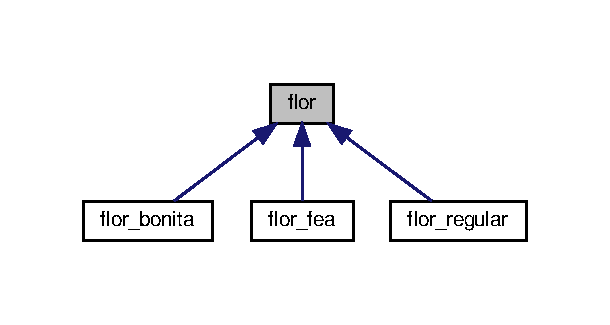
\includegraphics[width=293pt]{classflor__inherit__graph}
\end{center}
\end{figure}
\subsection*{Métodos públicos}
\begin{DoxyCompactItemize}
\item 
virtual void \hyperlink{classflor_a5fd1bd8f51024b772a5da6c0f6c8e9e2}{drawn} (\hyperlink{classplano}{plano} T, int x, int y)=0
\end{DoxyCompactItemize}
\subsection*{Atributos protegidos}
\begin{DoxyCompactItemize}
\item 
\mbox{\Hypertarget{classflor_ae973a3f5eedbeed6fa48e71743b9d6f3}\label{classflor_ae973a3f5eedbeed6fa48e71743b9d6f3}} 
int {\bfseries petalos}
\end{DoxyCompactItemize}


\subsection{Descripción detallada}
La clase flor contiene la funcion drawn para poder dibujarlo en pantalla  Se instancia el dato miembro. 

\subsection{Documentación de las funciones miembro}
\mbox{\Hypertarget{classflor_a5fd1bd8f51024b772a5da6c0f6c8e9e2}\label{classflor_a5fd1bd8f51024b772a5da6c0f6c8e9e2}} 
\index{flor@{flor}!drawn@{drawn}}
\index{drawn@{drawn}!flor@{flor}}
\subsubsection{\texorpdfstring{drawn()}{drawn()}}
{\footnotesize\ttfamily virtual void flor\+::drawn (\begin{DoxyParamCaption}\item[{\hyperlink{classplano}{plano}}]{T,  }\item[{int}]{x,  }\item[{int}]{y }\end{DoxyParamCaption})\hspace{0.3cm}{\ttfamily [pure virtual]}}

drawn. La funcion drawn es virtual para que sus hijas puedan sobreescribirla de acuerdo a lo que cada una quiera. 

Implementado en \hyperlink{classflor__regular_a5805895cf36946a69173b64aaf504c58}{flor\+\_\+regular}, \hyperlink{classflor__fea_af4ee97eef5e4ac46e5fbafb737759c3b}{flor\+\_\+fea} y \hyperlink{classflor__bonita_a25162281fab0a1118962f1db69b4fa81}{flor\+\_\+bonita}.



La documentación para esta clase fue generada a partir del siguiente fichero\+:\begin{DoxyCompactItemize}
\item 
\hyperlink{factory__method__flor_8h}{factory\+\_\+method\+\_\+flor.\+h}\end{DoxyCompactItemize}

\hypertarget{classflor__bonita}{}\section{Referencia de la Clase flor\+\_\+bonita}
\label{classflor__bonita}\index{flor\+\_\+bonita@{flor\+\_\+bonita}}


La clase \hyperlink{classflor__bonita}{flor\+\_\+bonita} es un tipo de flor en la que su dibujo es bonito,contiene la funcion drawn para poder visualizarlo, hereda de la clase flor  Se tiene constructor y destructor.  




{\ttfamily \#include $<$factory\+\_\+method\+\_\+flor.\+h$>$}



Diagrama de herencias de flor\+\_\+bonita
\nopagebreak
\begin{figure}[H]
\begin{center}
\leavevmode
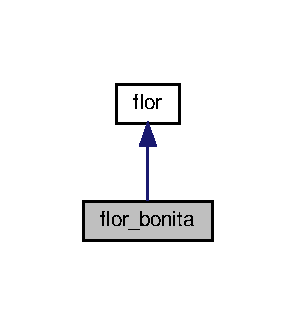
\includegraphics[width=142pt]{classflor__bonita__inherit__graph}
\end{center}
\end{figure}


Diagrama de colaboración para flor\+\_\+bonita\+:
\nopagebreak
\begin{figure}[H]
\begin{center}
\leavevmode
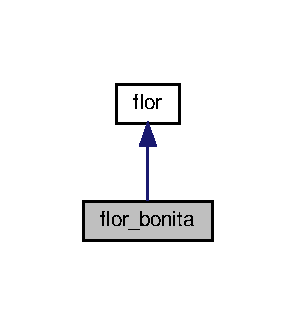
\includegraphics[width=142pt]{classflor__bonita__coll__graph}
\end{center}
\end{figure}
\subsection*{Métodos públicos}
\begin{DoxyCompactItemize}
\item 
\hyperlink{classflor__bonita_a650112410a675dce9b0e4c91d6182265}{flor\+\_\+bonita} (int n\+\_\+petalos)
\item 
\hyperlink{classflor__bonita_a56aa0024af8048194fa6400832ef7f97}{$\sim$flor\+\_\+bonita} ()
\item 
void \hyperlink{classflor__bonita_a25162281fab0a1118962f1db69b4fa81}{drawn} (\hyperlink{classplano}{plano} p, int x, int y)
\end{DoxyCompactItemize}
\subsection*{Otros miembros heredados}


\subsection{Descripción detallada}
La clase \hyperlink{classflor__bonita}{flor\+\_\+bonita} es un tipo de flor en la que su dibujo es bonito,contiene la funcion drawn para poder visualizarlo, hereda de la clase flor  Se tiene constructor y destructor. 

\subsection{Documentación del constructor y destructor}
\mbox{\Hypertarget{classflor__bonita_a650112410a675dce9b0e4c91d6182265}\label{classflor__bonita_a650112410a675dce9b0e4c91d6182265}} 
\index{flor\+\_\+bonita@{flor\+\_\+bonita}!flor\+\_\+bonita@{flor\+\_\+bonita}}
\index{flor\+\_\+bonita@{flor\+\_\+bonita}!flor\+\_\+bonita@{flor\+\_\+bonita}}
\subsubsection{\texorpdfstring{flor\+\_\+bonita()}{flor\_bonita()}}
{\footnotesize\ttfamily flor\+\_\+bonita\+::flor\+\_\+bonita (\begin{DoxyParamCaption}\item[{int}]{n\+\_\+petalos }\end{DoxyParamCaption})}

Constructor. 
\begin{DoxyParams}{Parámetros}
{\em n\+\_\+petalos} & es la cantidad de petalos que tiene la flor. \\
\hline
\end{DoxyParams}
\mbox{\Hypertarget{classflor__bonita_a56aa0024af8048194fa6400832ef7f97}\label{classflor__bonita_a56aa0024af8048194fa6400832ef7f97}} 
\index{flor\+\_\+bonita@{flor\+\_\+bonita}!````~flor\+\_\+bonita@{$\sim$flor\+\_\+bonita}}
\index{````~flor\+\_\+bonita@{$\sim$flor\+\_\+bonita}!flor\+\_\+bonita@{flor\+\_\+bonita}}
\subsubsection{\texorpdfstring{$\sim$flor\+\_\+bonita()}{~flor\_bonita()}}
{\footnotesize\ttfamily flor\+\_\+bonita\+::$\sim$flor\+\_\+bonita (\begin{DoxyParamCaption}{ }\end{DoxyParamCaption})}

Destructor 

\subsection{Documentación de las funciones miembro}
\mbox{\Hypertarget{classflor__bonita_a25162281fab0a1118962f1db69b4fa81}\label{classflor__bonita_a25162281fab0a1118962f1db69b4fa81}} 
\index{flor\+\_\+bonita@{flor\+\_\+bonita}!drawn@{drawn}}
\index{drawn@{drawn}!flor\+\_\+bonita@{flor\+\_\+bonita}}
\subsubsection{\texorpdfstring{drawn()}{drawn()}}
{\footnotesize\ttfamily void flor\+\_\+bonita\+::drawn (\begin{DoxyParamCaption}\item[{\hyperlink{classplano}{plano}}]{p,  }\item[{int}]{x,  }\item[{int}]{y }\end{DoxyParamCaption})\hspace{0.3cm}{\ttfamily [virtual]}}

La funcion drawn recibe el plano y las coordenadas donde se dibujará. 
\begin{DoxyParams}{Parámetros}
{\em p,nos} & permite hacer uso de la tortuga. \\
\hline
{\em x} & es la coordenada x en la que se dibujará. \\
\hline
{\em y} & es la coordenada y en la que se dibujará. \\
\hline
\end{DoxyParams}


Implementa \hyperlink{classflor_a5fd1bd8f51024b772a5da6c0f6c8e9e2}{flor}.



La documentación para esta clase fue generada a partir de los siguientes ficheros\+:\begin{DoxyCompactItemize}
\item 
\hyperlink{factory__method__flor_8h}{factory\+\_\+method\+\_\+flor.\+h}\item 
\hyperlink{factory__method__flor_8cpp}{factory\+\_\+method\+\_\+flor.\+cpp}\end{DoxyCompactItemize}

\hypertarget{classflor__fea}{}\section{Referencia de la Clase flor\+\_\+fea}
\label{classflor__fea}\index{flor\+\_\+fea@{flor\+\_\+fea}}


La clase \hyperlink{classflor__fea}{flor\+\_\+fea} es un tipo de flor en la que su dibujo es feo,contiene la funcion drawn para poder visualizarlo, hereda de la clase flor  Se instancia el dato miembro.  




{\ttfamily \#include $<$factory\+\_\+method\+\_\+flor.\+h$>$}



Diagrama de herencias de flor\+\_\+fea
\nopagebreak
\begin{figure}[H]
\begin{center}
\leavevmode
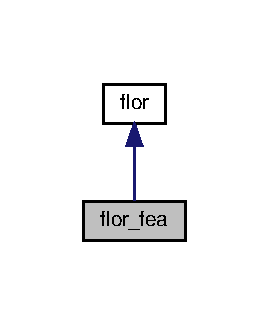
\includegraphics[width=129pt]{classflor__fea__inherit__graph}
\end{center}
\end{figure}


Diagrama de colaboración para flor\+\_\+fea\+:
\nopagebreak
\begin{figure}[H]
\begin{center}
\leavevmode
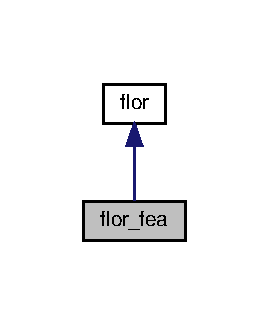
\includegraphics[width=129pt]{classflor__fea__coll__graph}
\end{center}
\end{figure}
\subsection*{Métodos públicos}
\begin{DoxyCompactItemize}
\item 
\hyperlink{classflor__fea_a617be6f164203d33d5f6da3926951d65}{flor\+\_\+fea} (int n\+\_\+petalos)
\item 
\hyperlink{classflor__fea_afafbf5440bec15a1fde668e1be42d42e}{$\sim$flor\+\_\+fea} ()
\item 
void \hyperlink{classflor__fea_af4ee97eef5e4ac46e5fbafb737759c3b}{drawn} (\hyperlink{classplano}{plano} p, int x, int y)
\end{DoxyCompactItemize}
\subsection*{Otros miembros heredados}


\subsection{Descripción detallada}
La clase \hyperlink{classflor__fea}{flor\+\_\+fea} es un tipo de flor en la que su dibujo es feo,contiene la funcion drawn para poder visualizarlo, hereda de la clase flor  Se instancia el dato miembro. 

\subsection{Documentación del constructor y destructor}
\mbox{\Hypertarget{classflor__fea_a617be6f164203d33d5f6da3926951d65}\label{classflor__fea_a617be6f164203d33d5f6da3926951d65}} 
\index{flor\+\_\+fea@{flor\+\_\+fea}!flor\+\_\+fea@{flor\+\_\+fea}}
\index{flor\+\_\+fea@{flor\+\_\+fea}!flor\+\_\+fea@{flor\+\_\+fea}}
\subsubsection{\texorpdfstring{flor\+\_\+fea()}{flor\_fea()}}
{\footnotesize\ttfamily flor\+\_\+fea\+::flor\+\_\+fea (\begin{DoxyParamCaption}\item[{int}]{n\+\_\+petalos }\end{DoxyParamCaption})}

Constructor. 
\begin{DoxyParams}{Parámetros}
{\em n\+\_\+petalos} & es la cantidad de petalos que tiene la flor. \\
\hline
\end{DoxyParams}
\mbox{\Hypertarget{classflor__fea_afafbf5440bec15a1fde668e1be42d42e}\label{classflor__fea_afafbf5440bec15a1fde668e1be42d42e}} 
\index{flor\+\_\+fea@{flor\+\_\+fea}!````~flor\+\_\+fea@{$\sim$flor\+\_\+fea}}
\index{````~flor\+\_\+fea@{$\sim$flor\+\_\+fea}!flor\+\_\+fea@{flor\+\_\+fea}}
\subsubsection{\texorpdfstring{$\sim$flor\+\_\+fea()}{~flor\_fea()}}
{\footnotesize\ttfamily flor\+\_\+fea\+::$\sim$flor\+\_\+fea (\begin{DoxyParamCaption}{ }\end{DoxyParamCaption})}

Destructor 

\subsection{Documentación de las funciones miembro}
\mbox{\Hypertarget{classflor__fea_af4ee97eef5e4ac46e5fbafb737759c3b}\label{classflor__fea_af4ee97eef5e4ac46e5fbafb737759c3b}} 
\index{flor\+\_\+fea@{flor\+\_\+fea}!drawn@{drawn}}
\index{drawn@{drawn}!flor\+\_\+fea@{flor\+\_\+fea}}
\subsubsection{\texorpdfstring{drawn()}{drawn()}}
{\footnotesize\ttfamily void flor\+\_\+fea\+::drawn (\begin{DoxyParamCaption}\item[{\hyperlink{classplano}{plano}}]{p,  }\item[{int}]{x,  }\item[{int}]{y }\end{DoxyParamCaption})\hspace{0.3cm}{\ttfamily [virtual]}}

La funcion drawn recibe el plano y las coordenadas donde se dibujará. 
\begin{DoxyParams}{Parámetros}
{\em p,nos} & permite hacer uso de la tortuga. \\
\hline
{\em x} & es la coordenada x en la que se dibujará. \\
\hline
{\em y} & es la coordenada y en la que se dibujará. \\
\hline
\end{DoxyParams}


Implementa \hyperlink{classflor_a5fd1bd8f51024b772a5da6c0f6c8e9e2}{flor}.



La documentación para esta clase fue generada a partir de los siguientes ficheros\+:\begin{DoxyCompactItemize}
\item 
\hyperlink{factory__method__flor_8h}{factory\+\_\+method\+\_\+flor.\+h}\item 
\hyperlink{factory__method__flor_8cpp}{factory\+\_\+method\+\_\+flor.\+cpp}\end{DoxyCompactItemize}

\hypertarget{classflor__regular}{}\section{Referencia de la Clase flor\+\_\+regular}
\label{classflor__regular}\index{flor\+\_\+regular@{flor\+\_\+regular}}


La clase \hyperlink{classflor__regular}{flor\+\_\+regular} es un tipo de flor en la que su dibujo es \hyperlink{classflor__regular}{flor\+\_\+regular},contiene la funcion drawn para poder visualizarlo, hereda de la clase flor  Se instancia el dato miembro.  




{\ttfamily \#include $<$factory\+\_\+method\+\_\+flor.\+h$>$}



Diagrama de herencias de flor\+\_\+regular
\nopagebreak
\begin{figure}[H]
\begin{center}
\leavevmode
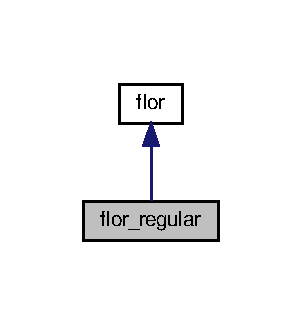
\includegraphics[width=145pt]{classflor__regular__inherit__graph}
\end{center}
\end{figure}


Diagrama de colaboración para flor\+\_\+regular\+:
\nopagebreak
\begin{figure}[H]
\begin{center}
\leavevmode
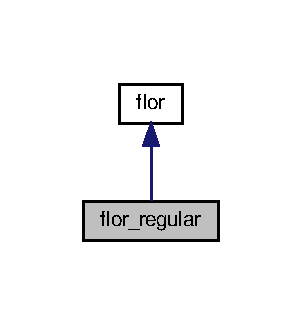
\includegraphics[width=145pt]{classflor__regular__coll__graph}
\end{center}
\end{figure}
\subsection*{Métodos públicos}
\begin{DoxyCompactItemize}
\item 
\hyperlink{classflor__regular_a299d17f2fed7eaae9db8f6a9533cff70}{flor\+\_\+regular} (int n\+\_\+petalos)
\item 
\hyperlink{classflor__regular_ae525b7823bdd11ad29908de8325af0eb}{$\sim$flor\+\_\+regular} ()
\item 
void \hyperlink{classflor__regular_a5805895cf36946a69173b64aaf504c58}{drawn} (\hyperlink{classplano}{plano} p, int x, int y)
\end{DoxyCompactItemize}
\subsection*{Otros miembros heredados}


\subsection{Descripción detallada}
La clase \hyperlink{classflor__regular}{flor\+\_\+regular} es un tipo de flor en la que su dibujo es \hyperlink{classflor__regular}{flor\+\_\+regular},contiene la funcion drawn para poder visualizarlo, hereda de la clase flor  Se instancia el dato miembro. 

\subsection{Documentación del constructor y destructor}
\mbox{\Hypertarget{classflor__regular_a299d17f2fed7eaae9db8f6a9533cff70}\label{classflor__regular_a299d17f2fed7eaae9db8f6a9533cff70}} 
\index{flor\+\_\+regular@{flor\+\_\+regular}!flor\+\_\+regular@{flor\+\_\+regular}}
\index{flor\+\_\+regular@{flor\+\_\+regular}!flor\+\_\+regular@{flor\+\_\+regular}}
\subsubsection{\texorpdfstring{flor\+\_\+regular()}{flor\_regular()}}
{\footnotesize\ttfamily flor\+\_\+regular\+::flor\+\_\+regular (\begin{DoxyParamCaption}\item[{int}]{n\+\_\+petalos }\end{DoxyParamCaption})}

Constructor. 
\begin{DoxyParams}{Parámetros}
{\em n\+\_\+petalos} & es la cantidad de petalos que tiene la flor. \\
\hline
\end{DoxyParams}
\mbox{\Hypertarget{classflor__regular_ae525b7823bdd11ad29908de8325af0eb}\label{classflor__regular_ae525b7823bdd11ad29908de8325af0eb}} 
\index{flor\+\_\+regular@{flor\+\_\+regular}!````~flor\+\_\+regular@{$\sim$flor\+\_\+regular}}
\index{````~flor\+\_\+regular@{$\sim$flor\+\_\+regular}!flor\+\_\+regular@{flor\+\_\+regular}}
\subsubsection{\texorpdfstring{$\sim$flor\+\_\+regular()}{~flor\_regular()}}
{\footnotesize\ttfamily flor\+\_\+regular\+::$\sim$flor\+\_\+regular (\begin{DoxyParamCaption}{ }\end{DoxyParamCaption})}

Destructor 

\subsection{Documentación de las funciones miembro}
\mbox{\Hypertarget{classflor__regular_a5805895cf36946a69173b64aaf504c58}\label{classflor__regular_a5805895cf36946a69173b64aaf504c58}} 
\index{flor\+\_\+regular@{flor\+\_\+regular}!drawn@{drawn}}
\index{drawn@{drawn}!flor\+\_\+regular@{flor\+\_\+regular}}
\subsubsection{\texorpdfstring{drawn()}{drawn()}}
{\footnotesize\ttfamily void flor\+\_\+regular\+::drawn (\begin{DoxyParamCaption}\item[{\hyperlink{classplano}{plano}}]{p,  }\item[{int}]{x,  }\item[{int}]{y }\end{DoxyParamCaption})\hspace{0.3cm}{\ttfamily [virtual]}}

La funcion drawn recibe el plano y las coordenadas donde se dibujará. 
\begin{DoxyParams}{Parámetros}
{\em p,nos} & permite hacer uso de la tortuga. \\
\hline
{\em x} & es la coordenada x en la que se dibujará. \\
\hline
{\em y} & es la coordenada y en la que se dibujará. \\
\hline
\end{DoxyParams}


Implementa \hyperlink{classflor_a5fd1bd8f51024b772a5da6c0f6c8e9e2}{flor}.



La documentación para esta clase fue generada a partir de los siguientes ficheros\+:\begin{DoxyCompactItemize}
\item 
\hyperlink{factory__method__flor_8h}{factory\+\_\+method\+\_\+flor.\+h}\item 
\hyperlink{factory__method__flor_8cpp}{factory\+\_\+method\+\_\+flor.\+cpp}\end{DoxyCompactItemize}

\hypertarget{classhoja}{}\section{Referencia de la Clase hoja}
\label{classhoja}\index{hoja@{hoja}}


La clase hoja contiene la funcion drawn para poder dibujará  Se instancia el dato miembro.  




{\ttfamily \#include $<$builder\+\_\+arbol.\+h$>$}

\subsection*{Métodos públicos}
\begin{DoxyCompactItemize}
\item 
void \hyperlink{classhoja_a4210f1a7c6235aced08fc9817085dbe4}{drawn} (\hyperlink{classplano}{plano} p, int x, int y)
\end{DoxyCompactItemize}
\subsection*{Atributos públicos}
\begin{DoxyCompactItemize}
\item 
\mbox{\Hypertarget{classhoja_a63cb838e5ebc05e229393db711d43afe}\label{classhoja_a63cb838e5ebc05e229393db711d43afe}} 
int {\bfseries size}
\end{DoxyCompactItemize}


\subsection{Descripción detallada}
La clase hoja contiene la funcion drawn para poder dibujará  Se instancia el dato miembro. 

\subsection{Documentación de las funciones miembro}
\mbox{\Hypertarget{classhoja_a4210f1a7c6235aced08fc9817085dbe4}\label{classhoja_a4210f1a7c6235aced08fc9817085dbe4}} 
\index{hoja@{hoja}!drawn@{drawn}}
\index{drawn@{drawn}!hoja@{hoja}}
\subsubsection{\texorpdfstring{drawn()}{drawn()}}
{\footnotesize\ttfamily void hoja\+::drawn (\begin{DoxyParamCaption}\item[{\hyperlink{classplano}{plano}}]{p,  }\item[{int}]{x,  }\item[{int}]{y }\end{DoxyParamCaption})}

La funcion drawn recibe el plano y las coordenadas donde se dibujará. 
\begin{DoxyParams}{Parámetros}
{\em p,nos} & permite hacer uso de la tortuga. \\
\hline
{\em x} & es la coordenada x en la que se dibujará. \\
\hline
{\em y} & es la coordenada y en la que se dibujará. \\
\hline
\end{DoxyParams}


La documentación para esta clase fue generada a partir de los siguientes ficheros\+:\begin{DoxyCompactItemize}
\item 
\hyperlink{builder__arbol_8h}{builder\+\_\+arbol.\+h}\item 
\hyperlink{builder__arbol_8cpp}{builder\+\_\+arbol.\+cpp}\end{DoxyCompactItemize}

\hypertarget{classnieve}{}\section{Referencia de la Clase nieve}
\label{classnieve}\index{nieve@{nieve}}


La clase nieve es la clase que crea las particulas de nieve.  Se instancia el dato miembro.  




{\ttfamily \#include $<$flyweight\+\_\+nieve.\+h$>$}

\subsection*{Métodos públicos}
\begin{DoxyCompactItemize}
\item 
\hyperlink{classnieve_acb9180479e9ef3330c9794a4fb69831a}{nieve} (int cantidad=3, int tam=5)
\item 
\hyperlink{classnieve_a554baea3727dc5650c5e8cec2f765e24}{$\sim$nieve} ()
\item 
void \hyperlink{classnieve_a0b49a0d373b8d3129fa11137ff6ce3e4}{drawn} (\hyperlink{classplano}{plano} p)
\item 
void \hyperlink{classnieve_a447ff743623611b1dd3bfe617e40d52e}{set\+\_\+cantidad} (int \+\_\+cant)
\item 
void \hyperlink{classnieve_a61ec704dc78cefdb6da47a8d24c59646}{add\+\_\+copo} (int tam)
\end{DoxyCompactItemize}


\subsection{Descripción detallada}
La clase nieve es la clase que crea las particulas de nieve.  Se instancia el dato miembro. 

\subsection{Documentación del constructor y destructor}
\mbox{\Hypertarget{classnieve_acb9180479e9ef3330c9794a4fb69831a}\label{classnieve_acb9180479e9ef3330c9794a4fb69831a}} 
\index{nieve@{nieve}!nieve@{nieve}}
\index{nieve@{nieve}!nieve@{nieve}}
\subsubsection{\texorpdfstring{nieve()}{nieve()}}
{\footnotesize\ttfamily nieve\+::nieve (\begin{DoxyParamCaption}\item[{int}]{cantidad = {\ttfamily 3},  }\item[{int}]{tam = {\ttfamily 5} }\end{DoxyParamCaption})}

Constructor. 
\begin{DoxyParams}{Parámetros}
{\em tam} & es el tamaño de cada copo de nieve. \\
\hline
{\em cantidad} & es la cantidad de nieve que sera creada. \\
\hline
\end{DoxyParams}
\mbox{\Hypertarget{classnieve_a554baea3727dc5650c5e8cec2f765e24}\label{classnieve_a554baea3727dc5650c5e8cec2f765e24}} 
\index{nieve@{nieve}!````~nieve@{$\sim$nieve}}
\index{````~nieve@{$\sim$nieve}!nieve@{nieve}}
\subsubsection{\texorpdfstring{$\sim$nieve()}{~nieve()}}
{\footnotesize\ttfamily nieve\+::$\sim$nieve (\begin{DoxyParamCaption}{ }\end{DoxyParamCaption})}

Destructor. 

\subsection{Documentación de las funciones miembro}
\mbox{\Hypertarget{classnieve_a61ec704dc78cefdb6da47a8d24c59646}\label{classnieve_a61ec704dc78cefdb6da47a8d24c59646}} 
\index{nieve@{nieve}!add\+\_\+copo@{add\+\_\+copo}}
\index{add\+\_\+copo@{add\+\_\+copo}!nieve@{nieve}}
\subsubsection{\texorpdfstring{add\+\_\+copo()}{add\_copo()}}
{\footnotesize\ttfamily void nieve\+::add\+\_\+copo (\begin{DoxyParamCaption}\item[{int}]{tam }\end{DoxyParamCaption})}

La funcion add\+\_\+copo añade un copo al vector de copos de nieve. 
\begin{DoxyParams}{Parámetros}
{\em tam} & es el tamaño de la punta del copo. \\
\hline
\end{DoxyParams}
\mbox{\Hypertarget{classnieve_a0b49a0d373b8d3129fa11137ff6ce3e4}\label{classnieve_a0b49a0d373b8d3129fa11137ff6ce3e4}} 
\index{nieve@{nieve}!drawn@{drawn}}
\index{drawn@{drawn}!nieve@{nieve}}
\subsubsection{\texorpdfstring{drawn()}{drawn()}}
{\footnotesize\ttfamily void nieve\+::drawn (\begin{DoxyParamCaption}\item[{\hyperlink{classplano}{plano}}]{p }\end{DoxyParamCaption})}

La funcion draw dibuja recibiento el plano en el que dibujar toda la nieve, en coordenadas aleatorias. 
\begin{DoxyParams}{Parámetros}
{\em p} & es el plano en el que se dibujara. \\
\hline
\end{DoxyParams}
\mbox{\Hypertarget{classnieve_a447ff743623611b1dd3bfe617e40d52e}\label{classnieve_a447ff743623611b1dd3bfe617e40d52e}} 
\index{nieve@{nieve}!set\+\_\+cantidad@{set\+\_\+cantidad}}
\index{set\+\_\+cantidad@{set\+\_\+cantidad}!nieve@{nieve}}
\subsubsection{\texorpdfstring{set\+\_\+cantidad()}{set\_cantidad()}}
{\footnotesize\ttfamily void nieve\+::set\+\_\+cantidad (\begin{DoxyParamCaption}\item[{int}]{\+\_\+cant }\end{DoxyParamCaption})}

La funcion set\+\_\+cantidad define la cantidad de copos de nieve que habra en el plano. 
\begin{DoxyParams}{Parámetros}
{\em \+\_\+cant} & la cantidad de copos de nieve. \\
\hline
\end{DoxyParams}


La documentación para esta clase fue generada a partir de los siguientes ficheros\+:\begin{DoxyCompactItemize}
\item 
\hyperlink{flyweight__nieve_8h}{flyweight\+\_\+nieve.\+h}\item 
\hyperlink{flyweight__nieve_8cpp}{flyweight\+\_\+nieve.\+cpp}\end{DoxyCompactItemize}

\hypertarget{classpaint1}{}\section{Referencia de la Clase paint1}
\label{classpaint1}\index{paint1@{paint1}}


La clase \hyperlink{classpaint1}{paint1} es un tipo de paint que tiene a arboles y a flores y tambien niev  Se instancia el dato miembro.  




{\ttfamily \#include $<$Abstract.\+h$>$}



Diagrama de herencias de paint1
\nopagebreak
\begin{figure}[H]
\begin{center}
\leavevmode
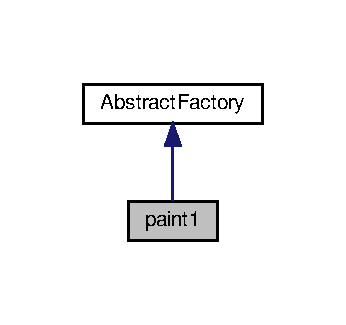
\includegraphics[width=166pt]{classpaint1__inherit__graph}
\end{center}
\end{figure}


Diagrama de colaboración para paint1\+:
\nopagebreak
\begin{figure}[H]
\begin{center}
\leavevmode
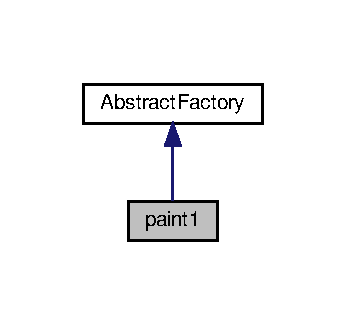
\includegraphics[width=166pt]{classpaint1__coll__graph}
\end{center}
\end{figure}
\subsection*{Métodos públicos}
\begin{DoxyCompactItemize}
\item 
\hyperlink{classarbol}{arbol} $\ast$ \hyperlink{classpaint1_a249b589508df7acb5e763abd1cae42c2}{getarbol} ()
\item 
\hyperlink{classflor}{flor} $\ast$ \hyperlink{classpaint1_ae5bf28220e7c9b9f8ce361de3feb5f39}{get\+Flor} ()
\item 
\hyperlink{classnieve}{nieve} $\ast$ \hyperlink{classpaint1_a402a3a74abf9644ba7a19fbb0e97ea4f}{getnieve} ()
\end{DoxyCompactItemize}


\subsection{Descripción detallada}
La clase \hyperlink{classpaint1}{paint1} es un tipo de paint que tiene a arboles y a flores y tambien niev  Se instancia el dato miembro. 

\subsection{Documentación de las funciones miembro}
\mbox{\Hypertarget{classpaint1_a249b589508df7acb5e763abd1cae42c2}\label{classpaint1_a249b589508df7acb5e763abd1cae42c2}} 
\index{paint1@{paint1}!getarbol@{getarbol}}
\index{getarbol@{getarbol}!paint1@{paint1}}
\subsubsection{\texorpdfstring{getarbol()}{getarbol()}}
{\footnotesize\ttfamily \hyperlink{classarbol}{arbol} $\ast$ paint1\+::getarbol (\begin{DoxyParamCaption}{ }\end{DoxyParamCaption})\hspace{0.3cm}{\ttfamily [virtual]}}

La funcion \hyperlink{classpaint1_a249b589508df7acb5e763abd1cae42c2}{getarbol()} es la que me devuelve el arbol. 

Implementa \hyperlink{classAbstractFactory}{Abstract\+Factory}.

\mbox{\Hypertarget{classpaint1_ae5bf28220e7c9b9f8ce361de3feb5f39}\label{classpaint1_ae5bf28220e7c9b9f8ce361de3feb5f39}} 
\index{paint1@{paint1}!get\+Flor@{get\+Flor}}
\index{get\+Flor@{get\+Flor}!paint1@{paint1}}
\subsubsection{\texorpdfstring{get\+Flor()}{getFlor()}}
{\footnotesize\ttfamily \hyperlink{classflor}{flor} $\ast$ paint1\+::get\+Flor (\begin{DoxyParamCaption}{ }\end{DoxyParamCaption})\hspace{0.3cm}{\ttfamily [virtual]}}

La funcion \hyperlink{classpaint1_ae5bf28220e7c9b9f8ce361de3feb5f39}{get\+Flor()} es la que me devuelve la flor. 

Implementa \hyperlink{classAbstractFactory}{Abstract\+Factory}.

\mbox{\Hypertarget{classpaint1_a402a3a74abf9644ba7a19fbb0e97ea4f}\label{classpaint1_a402a3a74abf9644ba7a19fbb0e97ea4f}} 
\index{paint1@{paint1}!getnieve@{getnieve}}
\index{getnieve@{getnieve}!paint1@{paint1}}
\subsubsection{\texorpdfstring{getnieve()}{getnieve()}}
{\footnotesize\ttfamily \hyperlink{classnieve}{nieve} $\ast$ paint1\+::getnieve (\begin{DoxyParamCaption}{ }\end{DoxyParamCaption})\hspace{0.3cm}{\ttfamily [virtual]}}

La funcion \hyperlink{classpaint1_a402a3a74abf9644ba7a19fbb0e97ea4f}{getnieve()} es la que me devuelve la nieve. 

Implementa \hyperlink{classAbstractFactory}{Abstract\+Factory}.



La documentación para esta clase fue generada a partir de los siguientes ficheros\+:\begin{DoxyCompactItemize}
\item 
\hyperlink{Abstract_8h}{Abstract.\+h}\item 
\hyperlink{Abstract_8cpp}{Abstract.\+cpp}\end{DoxyCompactItemize}

\hypertarget{classpaint2}{}\section{Referencia de la Clase paint2}
\label{classpaint2}\index{paint2@{paint2}}


La clase \hyperlink{classpaint2}{paint2} es un tipo de paint que tiene a arboles y a flores y tambien nieve  Se instancia el dato miembro.  




{\ttfamily \#include $<$Abstract.\+h$>$}



Diagrama de herencias de paint2
\nopagebreak
\begin{figure}[H]
\begin{center}
\leavevmode
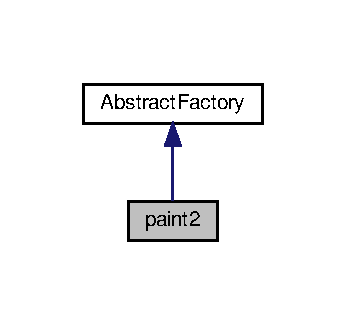
\includegraphics[width=166pt]{classpaint2__inherit__graph}
\end{center}
\end{figure}


Diagrama de colaboración para paint2\+:
\nopagebreak
\begin{figure}[H]
\begin{center}
\leavevmode
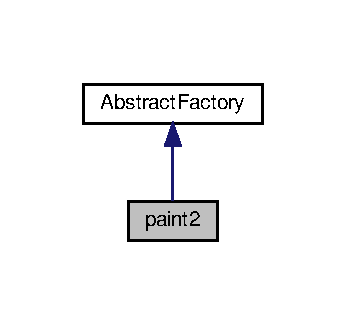
\includegraphics[width=166pt]{classpaint2__coll__graph}
\end{center}
\end{figure}
\subsection*{Métodos públicos}
\begin{DoxyCompactItemize}
\item 
\hyperlink{classarbol}{arbol} $\ast$ \hyperlink{classpaint2_a07e7d130f298e613dcdecf073acc8734}{getarbol} ()
\item 
\hyperlink{classflor}{flor} $\ast$ \hyperlink{classpaint2_af06042693fb9817ae4fa381a1d5699c9}{get\+Flor} ()
\item 
\hyperlink{classnieve}{nieve} $\ast$ \hyperlink{classpaint2_a0aeaabfae73dd3ddde19a6636c72732a}{getnieve} ()
\end{DoxyCompactItemize}


\subsection{Descripción detallada}
La clase \hyperlink{classpaint2}{paint2} es un tipo de paint que tiene a arboles y a flores y tambien nieve  Se instancia el dato miembro. 

\subsection{Documentación de las funciones miembro}
\mbox{\Hypertarget{classpaint2_a07e7d130f298e613dcdecf073acc8734}\label{classpaint2_a07e7d130f298e613dcdecf073acc8734}} 
\index{paint2@{paint2}!getarbol@{getarbol}}
\index{getarbol@{getarbol}!paint2@{paint2}}
\subsubsection{\texorpdfstring{getarbol()}{getarbol()}}
{\footnotesize\ttfamily \hyperlink{classarbol}{arbol} $\ast$ paint2\+::getarbol (\begin{DoxyParamCaption}{ }\end{DoxyParamCaption})\hspace{0.3cm}{\ttfamily [virtual]}}

La funcion \hyperlink{classpaint2_a07e7d130f298e613dcdecf073acc8734}{getarbol()} es la que me devuelve el arbol. 

Implementa \hyperlink{classAbstractFactory}{Abstract\+Factory}.

\mbox{\Hypertarget{classpaint2_af06042693fb9817ae4fa381a1d5699c9}\label{classpaint2_af06042693fb9817ae4fa381a1d5699c9}} 
\index{paint2@{paint2}!get\+Flor@{get\+Flor}}
\index{get\+Flor@{get\+Flor}!paint2@{paint2}}
\subsubsection{\texorpdfstring{get\+Flor()}{getFlor()}}
{\footnotesize\ttfamily \hyperlink{classflor}{flor} $\ast$ paint2\+::get\+Flor (\begin{DoxyParamCaption}{ }\end{DoxyParamCaption})\hspace{0.3cm}{\ttfamily [virtual]}}

La funcion \hyperlink{classpaint2_af06042693fb9817ae4fa381a1d5699c9}{get\+Flor()} es la que me devuelve la flor. 

Implementa \hyperlink{classAbstractFactory}{Abstract\+Factory}.

\mbox{\Hypertarget{classpaint2_a0aeaabfae73dd3ddde19a6636c72732a}\label{classpaint2_a0aeaabfae73dd3ddde19a6636c72732a}} 
\index{paint2@{paint2}!getnieve@{getnieve}}
\index{getnieve@{getnieve}!paint2@{paint2}}
\subsubsection{\texorpdfstring{getnieve()}{getnieve()}}
{\footnotesize\ttfamily \hyperlink{classnieve}{nieve} $\ast$ paint2\+::getnieve (\begin{DoxyParamCaption}{ }\end{DoxyParamCaption})\hspace{0.3cm}{\ttfamily [virtual]}}

La funcion \hyperlink{classpaint2_a0aeaabfae73dd3ddde19a6636c72732a}{getnieve()} es la que me devuelve la nieve. 

Implementa \hyperlink{classAbstractFactory}{Abstract\+Factory}.



La documentación para esta clase fue generada a partir de los siguientes ficheros\+:\begin{DoxyCompactItemize}
\item 
\hyperlink{Abstract_8h}{Abstract.\+h}\item 
\hyperlink{Abstract_8cpp}{Abstract.\+cpp}\end{DoxyCompactItemize}

\hypertarget{classparticles}{}\section{Referencia de la Clase particles}
\label{classparticles}\index{particles@{particles}}


La clase particles es la calse que dibuja solo una particula.  Se instancia el dato miembro.  




{\ttfamily \#include $<$flyweight\+\_\+nieve.\+h$>$}

\subsection*{Métodos públicos}
\begin{DoxyCompactItemize}
\item 
\hyperlink{classparticles_a3c777a01910495af29eba8f6716ff281}{particles} (int \+\_\+tam)
\item 
\hyperlink{classparticles_a595906f264178672e1f8fb3a047e056d}{$\sim$particles} ()
\item 
void \hyperlink{classparticles_a4ef23182e87e18e3cec15280478210d8}{set\+\_\+tam} (int tam)
\item 
void \hyperlink{classparticles_aed9719fe5f8de507f97c154b220307c6}{set\+\_\+x\+\_\+y} (int \+\_\+x, int \+\_\+y)
\item 
void \hyperlink{classparticles_a854301db81fec822416fa2a54a1b09d7}{drawn} (\hyperlink{classplano}{plano} p)
\end{DoxyCompactItemize}


\subsection{Descripción detallada}
La clase particles es la calse que dibuja solo una particula.  Se instancia el dato miembro. 

\subsection{Documentación del constructor y destructor}
\mbox{\Hypertarget{classparticles_a3c777a01910495af29eba8f6716ff281}\label{classparticles_a3c777a01910495af29eba8f6716ff281}} 
\index{particles@{particles}!particles@{particles}}
\index{particles@{particles}!particles@{particles}}
\subsubsection{\texorpdfstring{particles()}{particles()}}
{\footnotesize\ttfamily particles\+::particles (\begin{DoxyParamCaption}\item[{int}]{\+\_\+tam }\end{DoxyParamCaption})}

Constructor. 
\begin{DoxyParams}{Parámetros}
{\em \+\_\+tam} & es el tamaño del copo de nieve. \\
\hline
\end{DoxyParams}
\mbox{\Hypertarget{classparticles_a595906f264178672e1f8fb3a047e056d}\label{classparticles_a595906f264178672e1f8fb3a047e056d}} 
\index{particles@{particles}!````~particles@{$\sim$particles}}
\index{````~particles@{$\sim$particles}!particles@{particles}}
\subsubsection{\texorpdfstring{$\sim$particles()}{~particles()}}
{\footnotesize\ttfamily particles\+::$\sim$particles (\begin{DoxyParamCaption}{ }\end{DoxyParamCaption})}

Destructor. 

\subsection{Documentación de las funciones miembro}
\mbox{\Hypertarget{classparticles_a854301db81fec822416fa2a54a1b09d7}\label{classparticles_a854301db81fec822416fa2a54a1b09d7}} 
\index{particles@{particles}!drawn@{drawn}}
\index{drawn@{drawn}!particles@{particles}}
\subsubsection{\texorpdfstring{drawn()}{drawn()}}
{\footnotesize\ttfamily void particles\+::drawn (\begin{DoxyParamCaption}\item[{\hyperlink{classplano}{plano}}]{p }\end{DoxyParamCaption})}

La funcion drawn recibe el plano y se dibujará en las coordenadas ya establecidas. 
\begin{DoxyParams}{Parámetros}
{\em p} & nos permite hacer uso de la tortuga. \\
\hline
\end{DoxyParams}
\mbox{\Hypertarget{classparticles_a4ef23182e87e18e3cec15280478210d8}\label{classparticles_a4ef23182e87e18e3cec15280478210d8}} 
\index{particles@{particles}!set\+\_\+tam@{set\+\_\+tam}}
\index{set\+\_\+tam@{set\+\_\+tam}!particles@{particles}}
\subsubsection{\texorpdfstring{set\+\_\+tam()}{set\_tam()}}
{\footnotesize\ttfamily void particles\+::set\+\_\+tam (\begin{DoxyParamCaption}\item[{int}]{tam }\end{DoxyParamCaption})}

La funcion set\+\_\+tam le da un tamaño a la nieve. 
\begin{DoxyParams}{Parámetros}
{\em \+\_\+tam} & es el tamño que le das a la nieve \\
\hline
\end{DoxyParams}
\mbox{\Hypertarget{classparticles_aed9719fe5f8de507f97c154b220307c6}\label{classparticles_aed9719fe5f8de507f97c154b220307c6}} 
\index{particles@{particles}!set\+\_\+x\+\_\+y@{set\+\_\+x\+\_\+y}}
\index{set\+\_\+x\+\_\+y@{set\+\_\+x\+\_\+y}!particles@{particles}}
\subsubsection{\texorpdfstring{set\+\_\+x\+\_\+y()}{set\_x\_y()}}
{\footnotesize\ttfamily void particles\+::set\+\_\+x\+\_\+y (\begin{DoxyParamCaption}\item[{int}]{\+\_\+x,  }\item[{int}]{\+\_\+y }\end{DoxyParamCaption})}

La funcion set\+\_\+x\+\_\+y le da unas coordenadas a la nieve. 
\begin{DoxyParams}{Parámetros}
{\em \+\_\+x,\+\_\+y} & son las coordenadas x, y respectivamente. \\
\hline
\end{DoxyParams}


La documentación para esta clase fue generada a partir de los siguientes ficheros\+:\begin{DoxyCompactItemize}
\item 
\hyperlink{flyweight__nieve_8h}{flyweight\+\_\+nieve.\+h}\item 
\hyperlink{flyweight__nieve_8cpp}{flyweight\+\_\+nieve.\+cpp}\end{DoxyCompactItemize}

\hypertarget{classplano}{}\section{Referencia de la Clase plano}
\label{classplano}\index{plano@{plano}}


La clase plano tiene los elementos basicos para empezar a dibujar como se hace en la python turtle.  Definicion de la funciones usadas en la clase.  




{\ttfamily \#include $<$plano.\+h$>$}

\subsection*{Métodos públicos}
\begin{DoxyCompactItemize}
\item 
\hyperlink{classplano_a07a6173550219cbe2d32925afac542a5}{plano} (int width=500, int height=500)
\item 
void \hyperlink{classplano_a2febab8f233098b881ced3f4553526f2}{forward} (int cantidad)
\item 
void \hyperlink{classplano_ad5f11338792271b961051f7eff80c4cc}{left} (t\+\_\+coord grado)
\item 
void \hyperlink{classplano_a350bd814b14e4a876b601e608c4b7217}{right} (t\+\_\+coord grado)
\item 
void \hyperlink{classplano_a5758a4e96e2140941dd150e91e6029fd}{set\+\_\+color} (int R, int G, int B)
\item 
void \hyperlink{classplano_a48e4fbc9361ecaffe8a18545825ae19b}{penup} ()
\item 
void \hyperlink{classplano_aa2ae0a48000f85adfc61663ae7011aa2}{pendow} ()
\item 
void \hyperlink{classplano_a87e7fce6efc52d9b8c1e0c8946b1c2bb}{move} (t\+\_\+coord x, t\+\_\+coord y)
\item 
void \hyperlink{classplano_aa17e44a9925d265425e883f3bd8c1565}{display} (int argc, char $\ast$$\ast$argv)
\end{DoxyCompactItemize}


\subsection{Descripción detallada}
La clase plano tiene los elementos basicos para empezar a dibujar como se hace en la python turtle.  Definicion de la funciones usadas en la clase. 

\subsection{Documentación del constructor y destructor}
\mbox{\Hypertarget{classplano_a07a6173550219cbe2d32925afac542a5}\label{classplano_a07a6173550219cbe2d32925afac542a5}} 
\index{plano@{plano}!plano@{plano}}
\index{plano@{plano}!plano@{plano}}
\subsubsection{\texorpdfstring{plano()}{plano()}}
{\footnotesize\ttfamily plano\+::plano (\begin{DoxyParamCaption}\item[{int}]{width = {\ttfamily 500},  }\item[{int}]{height = {\ttfamily 500} }\end{DoxyParamCaption})}

Crear la turtle. por defecto se crea con w1=500 y h 
\begin{DoxyParams}{Parámetros}
{\em width,height} & coordinan el tamano del plano en el que se dibujara. \\
\hline
\end{DoxyParams}


\subsection{Documentación de las funciones miembro}
\mbox{\Hypertarget{classplano_aa17e44a9925d265425e883f3bd8c1565}\label{classplano_aa17e44a9925d265425e883f3bd8c1565}} 
\index{plano@{plano}!display@{display}}
\index{display@{display}!plano@{plano}}
\subsubsection{\texorpdfstring{display()}{display()}}
{\footnotesize\ttfamily void plano\+::display (\begin{DoxyParamCaption}\item[{int}]{argc,  }\item[{char $\ast$$\ast$}]{argv }\end{DoxyParamCaption})}

Muestra la ventana. 
\begin{DoxyParams}{Parámetros}
{\em argc,argv} & es necesario para la funcion glutopem\+Gl. \\
\hline
\end{DoxyParams}
\mbox{\Hypertarget{classplano_a2febab8f233098b881ced3f4553526f2}\label{classplano_a2febab8f233098b881ced3f4553526f2}} 
\index{plano@{plano}!forward@{forward}}
\index{forward@{forward}!plano@{plano}}
\subsubsection{\texorpdfstring{forward()}{forward()}}
{\footnotesize\ttfamily void plano\+::forward (\begin{DoxyParamCaption}\item[{int}]{cantidad }\end{DoxyParamCaption})}

Avanzar respecto al punto medio del plano. 
\begin{DoxyParams}{Parámetros}
{\em cantidad} & es la cantidad de pixeles que se avanzará. \\
\hline
\end{DoxyParams}
\mbox{\Hypertarget{classplano_ad5f11338792271b961051f7eff80c4cc}\label{classplano_ad5f11338792271b961051f7eff80c4cc}} 
\index{plano@{plano}!left@{left}}
\index{left@{left}!plano@{plano}}
\subsubsection{\texorpdfstring{left()}{left()}}
{\footnotesize\ttfamily void plano\+::left (\begin{DoxyParamCaption}\item[{t\+\_\+coord}]{grado }\end{DoxyParamCaption})}

Gira a la izquierda los grados que reciba respecto al punto en el que estes. 
\begin{DoxyParams}{Parámetros}
{\em grado,es} & la cantidad que se girara. \\
\hline
\end{DoxyParams}
\mbox{\Hypertarget{classplano_a87e7fce6efc52d9b8c1e0c8946b1c2bb}\label{classplano_a87e7fce6efc52d9b8c1e0c8946b1c2bb}} 
\index{plano@{plano}!move@{move}}
\index{move@{move}!plano@{plano}}
\subsubsection{\texorpdfstring{move()}{move()}}
{\footnotesize\ttfamily void plano\+::move (\begin{DoxyParamCaption}\item[{t\+\_\+coord}]{x,  }\item[{t\+\_\+coord}]{y }\end{DoxyParamCaption})}

Mueve la tortuga hace la coordenada (x, y). 
\begin{DoxyParams}{Parámetros}
{\em x,y} & funcionan como coordenadas. \\
\hline
\end{DoxyParams}
\mbox{\Hypertarget{classplano_aa2ae0a48000f85adfc61663ae7011aa2}\label{classplano_aa2ae0a48000f85adfc61663ae7011aa2}} 
\index{plano@{plano}!pendow@{pendow}}
\index{pendow@{pendow}!plano@{plano}}
\subsubsection{\texorpdfstring{pendow()}{pendow()}}
{\footnotesize\ttfamily void plano\+::pendow (\begin{DoxyParamCaption}{ }\end{DoxyParamCaption})}

La tortuga vuelve a pintar. \mbox{\Hypertarget{classplano_a48e4fbc9361ecaffe8a18545825ae19b}\label{classplano_a48e4fbc9361ecaffe8a18545825ae19b}} 
\index{plano@{plano}!penup@{penup}}
\index{penup@{penup}!plano@{plano}}
\subsubsection{\texorpdfstring{penup()}{penup()}}
{\footnotesize\ttfamily void plano\+::penup (\begin{DoxyParamCaption}{ }\end{DoxyParamCaption})}

La tortuga deja de pintar. \mbox{\Hypertarget{classplano_a350bd814b14e4a876b601e608c4b7217}\label{classplano_a350bd814b14e4a876b601e608c4b7217}} 
\index{plano@{plano}!right@{right}}
\index{right@{right}!plano@{plano}}
\subsubsection{\texorpdfstring{right()}{right()}}
{\footnotesize\ttfamily void plano\+::right (\begin{DoxyParamCaption}\item[{t\+\_\+coord}]{grado }\end{DoxyParamCaption})}

Gira a la derecha los grados que reciba respecto al punto en el que estes. 
\begin{DoxyParams}{Parámetros}
{\em grado,es} & la cantidad que se girara. \\
\hline
\end{DoxyParams}
\mbox{\Hypertarget{classplano_a5758a4e96e2140941dd150e91e6029fd}\label{classplano_a5758a4e96e2140941dd150e91e6029fd}} 
\index{plano@{plano}!set\+\_\+color@{set\+\_\+color}}
\index{set\+\_\+color@{set\+\_\+color}!plano@{plano}}
\subsubsection{\texorpdfstring{set\+\_\+color()}{set\_color()}}
{\footnotesize\ttfamily void plano\+::set\+\_\+color (\begin{DoxyParamCaption}\item[{int}]{R,  }\item[{int}]{G,  }\item[{int}]{B }\end{DoxyParamCaption})}

Define el color con el que se dibujara usa el formato R\+GB, que puede ir de 0-\/255. 
\begin{DoxyParams}{Parámetros}
{\em R,G,B} & inicializan el color de tipo R\+GB. \\
\hline
\end{DoxyParams}


La documentación para esta clase fue generada a partir de los siguientes ficheros\+:\begin{DoxyCompactItemize}
\item 
\hyperlink{plano_8h}{plano.\+h}\item 
\hyperlink{plano_8cpp}{plano.\+cpp}\end{DoxyCompactItemize}

\hypertarget{classrama}{}\section{Referencia de la Clase rama}
\label{classrama}\index{rama@{rama}}


La clase rama contiene la funcion drawn para poder dibujará.  Se instancia el dato miembro.  




{\ttfamily \#include $<$builder\+\_\+arbol.\+h$>$}

\subsection*{Métodos públicos}
\begin{DoxyCompactItemize}
\item 
void \hyperlink{classrama_a2b4b067ff7da51ec0db012b6162ab6f1}{drawn} (\hyperlink{classplano}{plano} p, int x, int y)
\end{DoxyCompactItemize}
\subsection*{Atributos públicos}
\begin{DoxyCompactItemize}
\item 
\mbox{\Hypertarget{classrama_a86bc8fa67daee270412e4b472ba24511}\label{classrama_a86bc8fa67daee270412e4b472ba24511}} 
int {\bfseries size}
\end{DoxyCompactItemize}


\subsection{Descripción detallada}
La clase rama contiene la funcion drawn para poder dibujará.  Se instancia el dato miembro. 

\subsection{Documentación de las funciones miembro}
\mbox{\Hypertarget{classrama_a2b4b067ff7da51ec0db012b6162ab6f1}\label{classrama_a2b4b067ff7da51ec0db012b6162ab6f1}} 
\index{rama@{rama}!drawn@{drawn}}
\index{drawn@{drawn}!rama@{rama}}
\subsubsection{\texorpdfstring{drawn()}{drawn()}}
{\footnotesize\ttfamily void rama\+::drawn (\begin{DoxyParamCaption}\item[{\hyperlink{classplano}{plano}}]{p,  }\item[{int}]{x,  }\item[{int}]{y }\end{DoxyParamCaption})}

La funcion drawn recibe el plano y las coordenadas donde se dibujará. 
\begin{DoxyParams}{Parámetros}
{\em p,nos} & permite hacer uso de la tortuga. \\
\hline
{\em x} & es la coordenada x en la que se dibujará. \\
\hline
{\em y} & es la coordenada y en la que se dibujará. \\
\hline
\end{DoxyParams}


La documentación para esta clase fue generada a partir de los siguientes ficheros\+:\begin{DoxyCompactItemize}
\item 
\hyperlink{builder__arbol_8h}{builder\+\_\+arbol.\+h}\item 
\hyperlink{builder__arbol_8cpp}{builder\+\_\+arbol.\+cpp}\end{DoxyCompactItemize}

\hypertarget{classsnow__flyweight}{}\section{Referencia de la Clase snow\+\_\+flyweight}
\label{classsnow__flyweight}\index{snow\+\_\+flyweight@{snow\+\_\+flyweight}}


La clase \hyperlink{classsnow__flyweight}{snow\+\_\+flyweight} es el singleton que dibuja la nieve.  Se instancia el dato miembro.  




{\ttfamily \#include $<$flyweight\+\_\+nieve.\+h$>$}



Diagrama de colaboración para snow\+\_\+flyweight\+:
\nopagebreak
\begin{figure}[H]
\begin{center}
\leavevmode
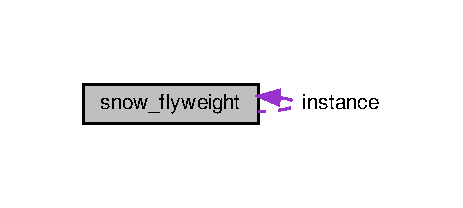
\includegraphics[width=222pt]{classsnow__flyweight__coll__graph}
\end{center}
\end{figure}
\subsection*{Métodos públicos}
\begin{DoxyCompactItemize}
\item 
void \hyperlink{classsnow__flyweight_aaf41210615d014dbd8d679cc7a48003e}{set\+\_\+tam} (int \+\_\+tam)
\item 
int \hyperlink{classsnow__flyweight_a64f410373e401b52629c93bf917b4b41}{get\+\_\+tam} ()
\end{DoxyCompactItemize}
\subsection*{Métodos públicos estáticos}
\begin{DoxyCompactItemize}
\item 
static \hyperlink{classsnow__flyweight}{snow\+\_\+flyweight} $\ast$ \hyperlink{classsnow__flyweight_a6035abfd67cce3ff166a5c9fc00e286c}{get\+\_\+instance} ()
\end{DoxyCompactItemize}
\subsection*{Atributos públicos estáticos}
\begin{DoxyCompactItemize}
\item 
\mbox{\Hypertarget{classsnow__flyweight_a88b4b4efea791663431768a955ef36f6}\label{classsnow__flyweight_a88b4b4efea791663431768a955ef36f6}} 
static \hyperlink{classsnow__flyweight}{snow\+\_\+flyweight} $\ast$ {\bfseries instance} =0
\end{DoxyCompactItemize}


\subsection{Descripción detallada}
La clase \hyperlink{classsnow__flyweight}{snow\+\_\+flyweight} es el singleton que dibuja la nieve.  Se instancia el dato miembro. 

\subsection{Documentación de las funciones miembro}
\mbox{\Hypertarget{classsnow__flyweight_a6035abfd67cce3ff166a5c9fc00e286c}\label{classsnow__flyweight_a6035abfd67cce3ff166a5c9fc00e286c}} 
\index{snow\+\_\+flyweight@{snow\+\_\+flyweight}!get\+\_\+instance@{get\+\_\+instance}}
\index{get\+\_\+instance@{get\+\_\+instance}!snow\+\_\+flyweight@{snow\+\_\+flyweight}}
\subsubsection{\texorpdfstring{get\+\_\+instance()}{get\_instance()}}
{\footnotesize\ttfamily \hyperlink{classsnow__flyweight}{snow\+\_\+flyweight} $\ast$ snow\+\_\+flyweight\+::get\+\_\+instance (\begin{DoxyParamCaption}{ }\end{DoxyParamCaption})\hspace{0.3cm}{\ttfamily [static]}}

La funcion get\+\_\+instance devuelve la nieve en singleton. \mbox{\Hypertarget{classsnow__flyweight_a64f410373e401b52629c93bf917b4b41}\label{classsnow__flyweight_a64f410373e401b52629c93bf917b4b41}} 
\index{snow\+\_\+flyweight@{snow\+\_\+flyweight}!get\+\_\+tam@{get\+\_\+tam}}
\index{get\+\_\+tam@{get\+\_\+tam}!snow\+\_\+flyweight@{snow\+\_\+flyweight}}
\subsubsection{\texorpdfstring{get\+\_\+tam()}{get\_tam()}}
{\footnotesize\ttfamily int snow\+\_\+flyweight\+::get\+\_\+tam (\begin{DoxyParamCaption}{ }\end{DoxyParamCaption})}

La funcion get\+\_\+tam devuelve el tamaño de la nieve. \mbox{\Hypertarget{classsnow__flyweight_aaf41210615d014dbd8d679cc7a48003e}\label{classsnow__flyweight_aaf41210615d014dbd8d679cc7a48003e}} 
\index{snow\+\_\+flyweight@{snow\+\_\+flyweight}!set\+\_\+tam@{set\+\_\+tam}}
\index{set\+\_\+tam@{set\+\_\+tam}!snow\+\_\+flyweight@{snow\+\_\+flyweight}}
\subsubsection{\texorpdfstring{set\+\_\+tam()}{set\_tam()}}
{\footnotesize\ttfamily void snow\+\_\+flyweight\+::set\+\_\+tam (\begin{DoxyParamCaption}\item[{int}]{\+\_\+tam }\end{DoxyParamCaption})}

La funcion set\+\_\+tam le da un tamaño a la nieve. 
\begin{DoxyParams}{Parámetros}
{\em \+\_\+tam} & es el tamño que le das a la nieve \\
\hline
\end{DoxyParams}


La documentación para esta clase fue generada a partir de los siguientes ficheros\+:\begin{DoxyCompactItemize}
\item 
\hyperlink{flyweight__nieve_8h}{flyweight\+\_\+nieve.\+h}\item 
\hyperlink{flyweight__nieve_8cpp}{flyweight\+\_\+nieve.\+cpp}\end{DoxyCompactItemize}

\hypertarget{classtronco}{}\section{Referencia de la Clase tronco}
\label{classtronco}\index{tronco@{tronco}}


La clase tronco contiene la funcion drawn para poder dibujarlo  Se instancia el dato miembro.  




{\ttfamily \#include $<$builder\+\_\+arbol.\+h$>$}

\subsection*{Métodos públicos}
\begin{DoxyCompactItemize}
\item 
void \hyperlink{classtronco_a8994db3bd2b43773f71311f2e0146e44}{drawn} (\hyperlink{classplano}{plano} p, int x, int y)
\end{DoxyCompactItemize}
\subsection*{Atributos públicos}
\begin{DoxyCompactItemize}
\item 
\mbox{\Hypertarget{classtronco_adc9931467b34c8d6436eb220d672d08d}\label{classtronco_adc9931467b34c8d6436eb220d672d08d}} 
int {\bfseries size}
\end{DoxyCompactItemize}


\subsection{Descripción detallada}
La clase tronco contiene la funcion drawn para poder dibujarlo  Se instancia el dato miembro. 

\subsection{Documentación de las funciones miembro}
\mbox{\Hypertarget{classtronco_a8994db3bd2b43773f71311f2e0146e44}\label{classtronco_a8994db3bd2b43773f71311f2e0146e44}} 
\index{tronco@{tronco}!drawn@{drawn}}
\index{drawn@{drawn}!tronco@{tronco}}
\subsubsection{\texorpdfstring{drawn()}{drawn()}}
{\footnotesize\ttfamily void tronco\+::drawn (\begin{DoxyParamCaption}\item[{\hyperlink{classplano}{plano}}]{p,  }\item[{int}]{x,  }\item[{int}]{y }\end{DoxyParamCaption})}

La funcion drawn recibe el plano y las coordenadas donde se dibujará. 
\begin{DoxyParams}{Parámetros}
{\em p,nos} & permite hacer uso de la tortuga. \\
\hline
{\em x} & es la coordenada x en la que se dibujará. \\
\hline
{\em y} & es la coordenada y en la que se dibujará. \\
\hline
\end{DoxyParams}


La documentación para esta clase fue generada a partir de los siguientes ficheros\+:\begin{DoxyCompactItemize}
\item 
\hyperlink{builder__arbol_8h}{builder\+\_\+arbol.\+h}\item 
\hyperlink{builder__arbol_8cpp}{builder\+\_\+arbol.\+cpp}\end{DoxyCompactItemize}

\chapter{Documentación de archivos}
\hypertarget{Abstract_8cpp}{}\section{Referencia del Archivo Abstract.\+cpp}
\label{Abstract_8cpp}\index{Abstract.\+cpp@{Abstract.\+cpp}}


implementacion de la clase paints para la creacion de paints en Glut Open\+GL  


{\ttfamily \#include \char`\"{}Abstract.\+h\char`\"{}}\newline
Dependencia gráfica adjunta para Abstract.\+cpp\+:
\nopagebreak
\begin{figure}[H]
\begin{center}
\leavevmode
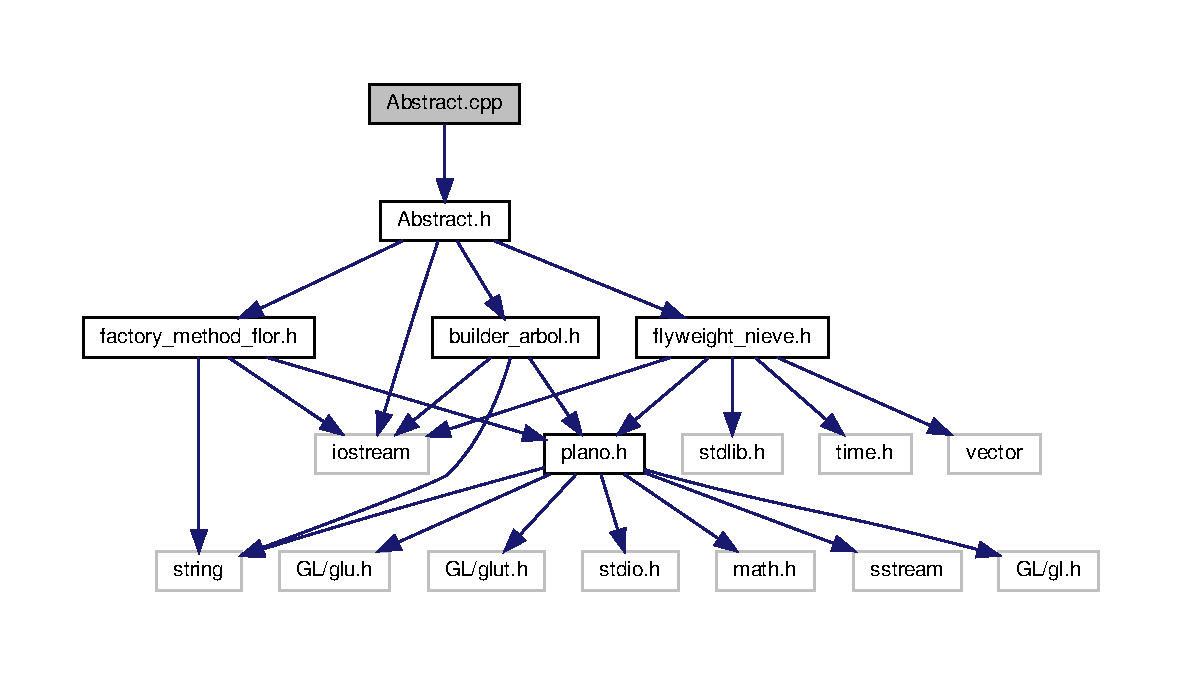
\includegraphics[width=350pt]{Abstract_8cpp__incl}
\end{center}
\end{figure}


\subsection{Descripción detallada}
implementacion de la clase paints para la creacion de paints en Glut Open\+GL 

\begin{DoxyAuthor}{Autor}
Walker Manrique 
\end{DoxyAuthor}
\begin{DoxyVersion}{Versión}
Revision 1.\+1 
\end{DoxyVersion}

\hypertarget{Abstract_8h}{}\section{Referencia del Archivo Abstract.\+h}
\label{Abstract_8h}\index{Abstract.\+h@{Abstract.\+h}}


implementacion de la clase paints para la creacion de paints en Glut Open\+GL  


{\ttfamily \#include $<$iostream$>$}\newline
{\ttfamily \#include \char`\"{}flyweight\+\_\+nieve.\+h\char`\"{}}\newline
{\ttfamily \#include \char`\"{}builder\+\_\+arbol.\+h\char`\"{}}\newline
{\ttfamily \#include \char`\"{}factory\+\_\+method\+\_\+flor.\+h\char`\"{}}\newline
Dependencia gráfica adjunta para Abstract.\+h\+:
\nopagebreak
\begin{figure}[H]
\begin{center}
\leavevmode
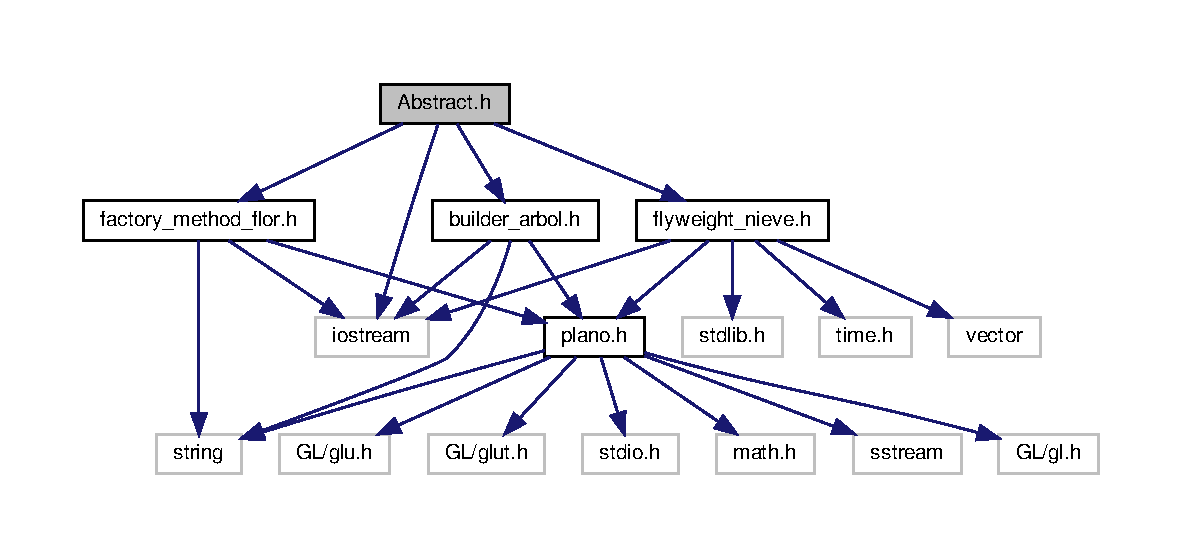
\includegraphics[width=350pt]{Abstract_8h__incl}
\end{center}
\end{figure}
Gráfico de los archivos que directa o indirectamente incluyen a este archivo\+:
\nopagebreak
\begin{figure}[H]
\begin{center}
\leavevmode
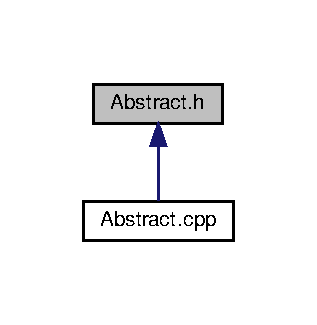
\includegraphics[width=152pt]{Abstract_8h__dep__incl}
\end{center}
\end{figure}
\subsection*{Clases}
\begin{DoxyCompactItemize}
\item 
class \hyperlink{classAbstractFactory}{Abstract\+Factory}
\begin{DoxyCompactList}\small\item\em La clase \hyperlink{classAbstractFactory}{Abstract\+Factory} contiene funciones para crear todo el paint  Se instancia el dato miembro. \end{DoxyCompactList}\item 
class \hyperlink{classpaint1}{paint1}
\begin{DoxyCompactList}\small\item\em La clase \hyperlink{classpaint1}{paint1} es un tipo de paint que tiene a arboles y a flores y tambien niev  Se instancia el dato miembro. \end{DoxyCompactList}\item 
class \hyperlink{classpaint2}{paint2}
\begin{DoxyCompactList}\small\item\em La clase \hyperlink{classpaint2}{paint2} es un tipo de paint que tiene a arboles y a flores y tambien nieve  Se instancia el dato miembro. \end{DoxyCompactList}\end{DoxyCompactItemize}


\subsection{Descripción detallada}
implementacion de la clase paints para la creacion de paints en Glut Open\+GL 

\begin{DoxyAuthor}{Autor}
Walker Manrique 
\end{DoxyAuthor}
\begin{DoxyVersion}{Versión}
Revision 1.\+1 
\end{DoxyVersion}

\hypertarget{builder__arbol_8cpp}{}\section{Referencia del Archivo builder\+\_\+arbol.\+cpp}
\label{builder__arbol_8cpp}\index{builder\+\_\+arbol.\+cpp@{builder\+\_\+arbol.\+cpp}}


implementacion de la clase arbol para la creacion de arboles en Glut Open\+GL  


{\ttfamily \#include \char`\"{}builder\+\_\+arbol.\+h\char`\"{}}\newline
Dependencia gráfica adjunta para builder\+\_\+arbol.\+cpp\+:
\nopagebreak
\begin{figure}[H]
\begin{center}
\leavevmode
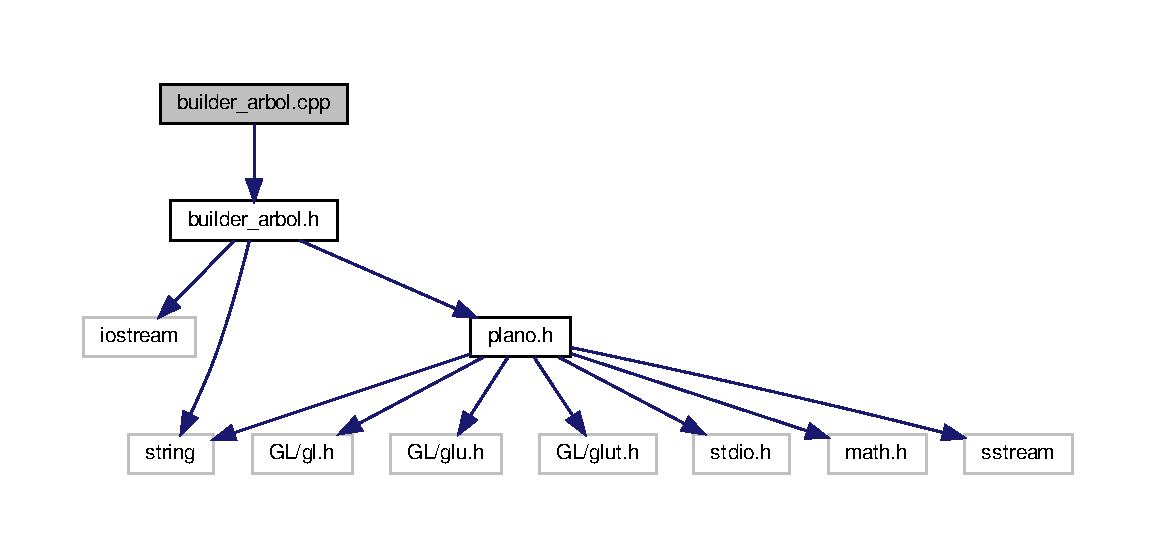
\includegraphics[width=350pt]{builder__arbol_8cpp__incl}
\end{center}
\end{figure}


\subsection{Descripción detallada}
implementacion de la clase arbol para la creacion de arboles en Glut Open\+GL 

\begin{DoxyAuthor}{Autor}
Walker Manrique 
\end{DoxyAuthor}
\begin{DoxyVersion}{Versión}
Revision 1.\+1 
\end{DoxyVersion}

\hypertarget{builder__arbol_8h}{}\section{Referencia del Archivo builder\+\_\+arbol.\+h}
\label{builder__arbol_8h}\index{builder\+\_\+arbol.\+h@{builder\+\_\+arbol.\+h}}


implementacion de la clase arbol para la creacion de arboles en Glut Open\+GL  


{\ttfamily \#include $<$iostream$>$}\newline
{\ttfamily \#include $<$string$>$}\newline
{\ttfamily \#include \char`\"{}plano.\+h\char`\"{}}\newline
Dependencia gráfica adjunta para builder\+\_\+arbol.\+h\+:
\nopagebreak
\begin{figure}[H]
\begin{center}
\leavevmode
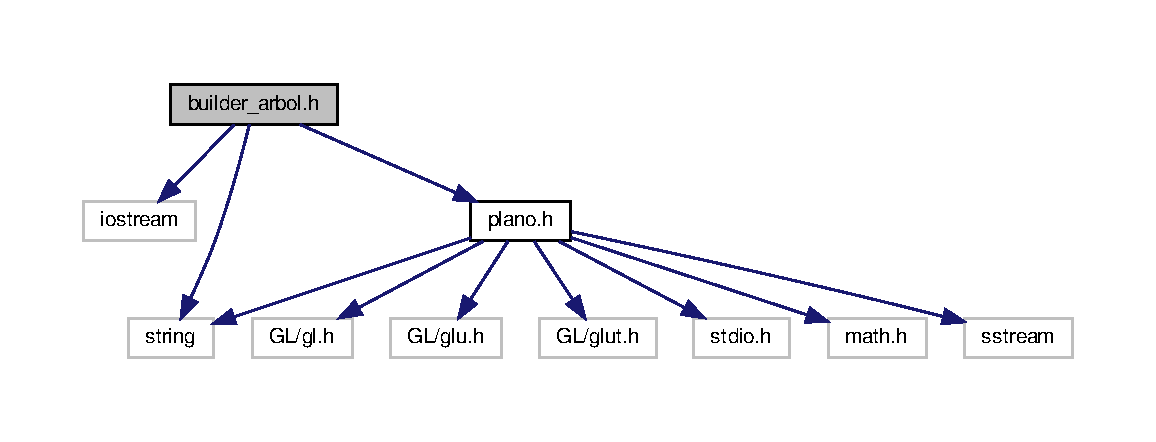
\includegraphics[width=350pt]{builder__arbol_8h__incl}
\end{center}
\end{figure}
Gráfico de los archivos que directa o indirectamente incluyen a este archivo\+:
\nopagebreak
\begin{figure}[H]
\begin{center}
\leavevmode
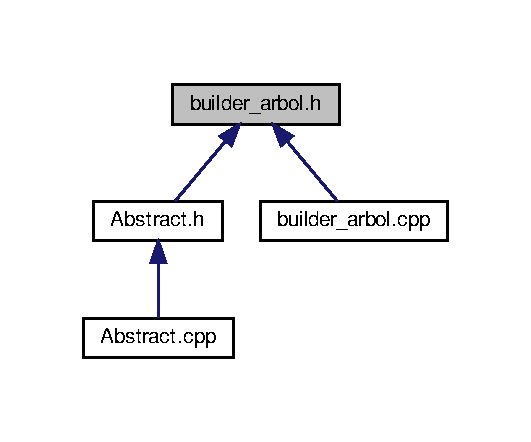
\includegraphics[width=255pt]{builder__arbol_8h__dep__incl}
\end{center}
\end{figure}
\subsection*{Clases}
\begin{DoxyCompactItemize}
\item 
class \hyperlink{classtronco}{tronco}
\begin{DoxyCompactList}\small\item\em La clase tronco contiene la funcion drawn para poder dibujarlo  Se instancia el dato miembro. \end{DoxyCompactList}\item 
class \hyperlink{classhoja}{hoja}
\begin{DoxyCompactList}\small\item\em La clase hoja contiene la funcion drawn para poder dibujará  Se instancia el dato miembro. \end{DoxyCompactList}\item 
class \hyperlink{classrama}{rama}
\begin{DoxyCompactList}\small\item\em La clase rama contiene la funcion drawn para poder dibujará.  Se instancia el dato miembro. \end{DoxyCompactList}\item 
class \hyperlink{classarbol}{arbol}
\begin{DoxyCompactList}\small\item\em La clase arbol contiene la funcion drawn para visualizar el arbol  Se instancia los datos miembros que son punteros a las partes del arbol. \end{DoxyCompactList}\item 
class \hyperlink{classbuilder}{builder}
\begin{DoxyCompactList}\small\item\em La clase builder contiene las funciones gettronco, gethojas, getramas para obtener las caracteristicas del arbol en sus clases hijas  Las funciones son virtual-\/puras y apuntan a las clases de las partes del arbol. \end{DoxyCompactList}\item 
class \hyperlink{classarbol__normal}{arbol\+\_\+normal}
\begin{DoxyCompactList}\small\item\em La clase \hyperlink{classarbol__normal}{arbol\+\_\+normal} hereda del arbol, estes es un arbol normal y unico. Tambien puede ser modificado.  Las funciones apuntan a las clases de las partes del arbol, asi como tambien son void. \end{DoxyCompactList}\item 
class \hyperlink{classdirector}{director}
\begin{DoxyCompactList}\small\item\em La clase director es la que crea mediante el builder o mediante parametros. \end{DoxyCompactList}\end{DoxyCompactItemize}


\subsection{Descripción detallada}
implementacion de la clase arbol para la creacion de arboles en Glut Open\+GL 

\begin{DoxyAuthor}{Autor}
Walker Manrique 
\end{DoxyAuthor}
\begin{DoxyVersion}{Versión}
Revision 1.\+1 
\end{DoxyVersion}

\hypertarget{factory__method__flor_8cpp}{}\section{Referencia del Archivo factory\+\_\+method\+\_\+flor.\+cpp}
\label{factory__method__flor_8cpp}\index{factory\+\_\+method\+\_\+flor.\+cpp@{factory\+\_\+method\+\_\+flor.\+cpp}}


implementacion de la clase flor para la creacion de flores en Glut Open\+GL  


{\ttfamily \#include \char`\"{}factory\+\_\+method\+\_\+flor.\+h\char`\"{}}\newline
Dependencia gráfica adjunta para factory\+\_\+method\+\_\+flor.\+cpp\+:
\nopagebreak
\begin{figure}[H]
\begin{center}
\leavevmode
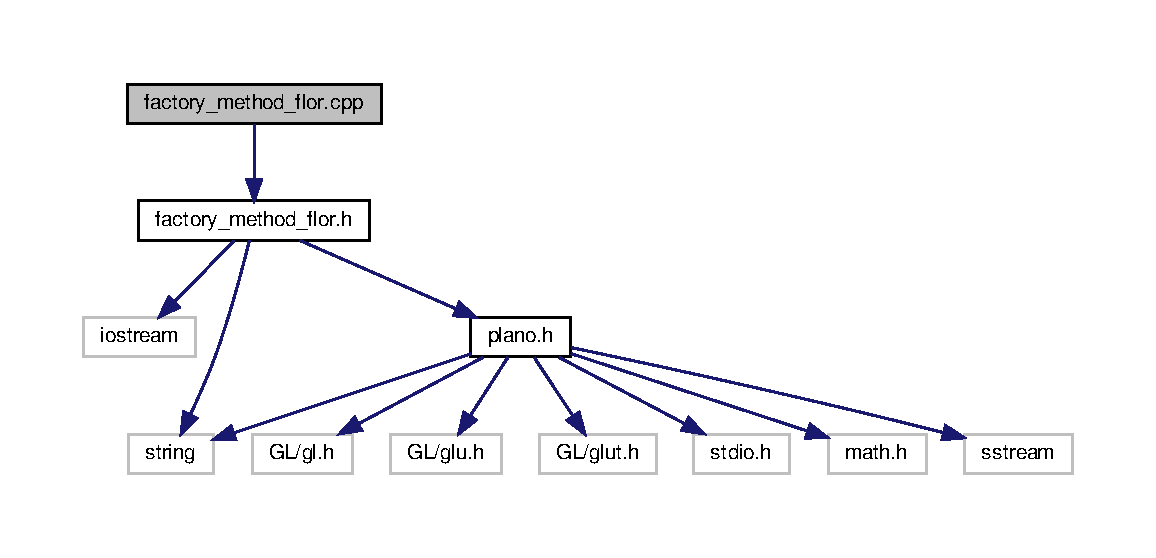
\includegraphics[width=350pt]{factory__method__flor_8cpp__incl}
\end{center}
\end{figure}


\subsection{Descripción detallada}
implementacion de la clase flor para la creacion de flores en Glut Open\+GL 

\begin{DoxyAuthor}{Autor}
Walker Manrique 
\end{DoxyAuthor}
\begin{DoxyVersion}{Versión}
Revision 1.\+1 
\end{DoxyVersion}

\hypertarget{factory__method__flor_8h}{}\section{Referencia del Archivo factory\+\_\+method\+\_\+flor.\+h}
\label{factory__method__flor_8h}\index{factory\+\_\+method\+\_\+flor.\+h@{factory\+\_\+method\+\_\+flor.\+h}}


implementacion de la clase flor para la creacion de flores en Glut Open\+GL  


{\ttfamily \#include $<$iostream$>$}\newline
{\ttfamily \#include $<$string$>$}\newline
{\ttfamily \#include \char`\"{}plano.\+h\char`\"{}}\newline
Dependencia gráfica adjunta para factory\+\_\+method\+\_\+flor.\+h\+:
\nopagebreak
\begin{figure}[H]
\begin{center}
\leavevmode
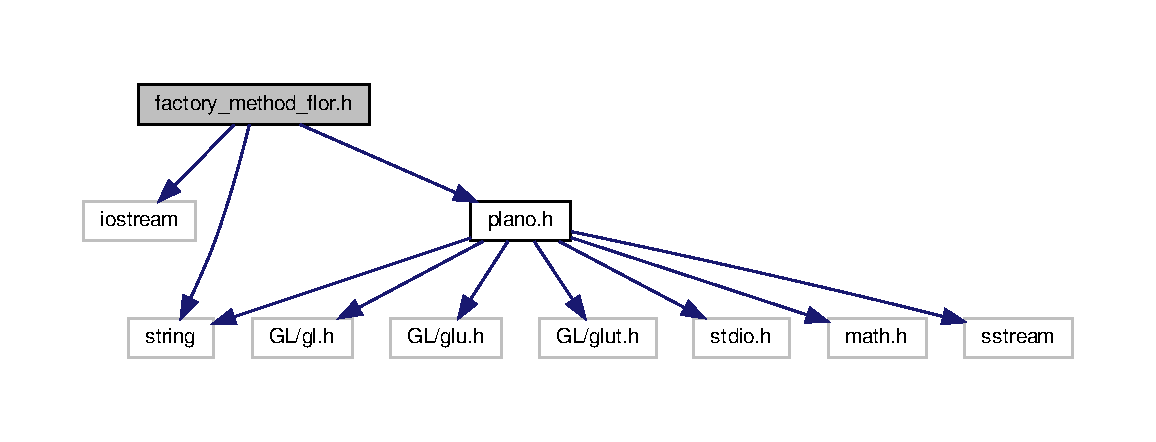
\includegraphics[width=350pt]{factory__method__flor_8h__incl}
\end{center}
\end{figure}
Gráfico de los archivos que directa o indirectamente incluyen a este archivo\+:
\nopagebreak
\begin{figure}[H]
\begin{center}
\leavevmode
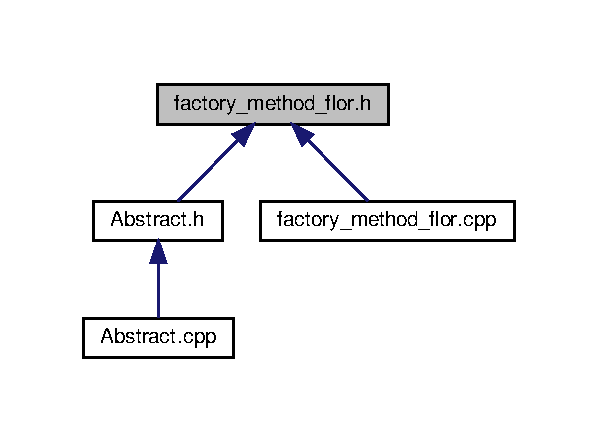
\includegraphics[width=287pt]{factory__method__flor_8h__dep__incl}
\end{center}
\end{figure}
\subsection*{Clases}
\begin{DoxyCompactItemize}
\item 
class \hyperlink{classflor}{flor}
\begin{DoxyCompactList}\small\item\em La clase flor contiene la funcion drawn para poder dibujarlo en pantalla  Se instancia el dato miembro. \end{DoxyCompactList}\item 
class \hyperlink{classflor__bonita}{flor\+\_\+bonita}
\begin{DoxyCompactList}\small\item\em La clase \hyperlink{classflor__bonita}{flor\+\_\+bonita} es un tipo de flor en la que su dibujo es bonito,contiene la funcion drawn para poder visualizarlo, hereda de la clase flor  Se tiene constructor y destructor. \end{DoxyCompactList}\item 
class \hyperlink{classflor__fea}{flor\+\_\+fea}
\begin{DoxyCompactList}\small\item\em La clase \hyperlink{classflor__fea}{flor\+\_\+fea} es un tipo de flor en la que su dibujo es feo,contiene la funcion drawn para poder visualizarlo, hereda de la clase flor  Se instancia el dato miembro. \end{DoxyCompactList}\item 
class \hyperlink{classflor__regular}{flor\+\_\+regular}
\begin{DoxyCompactList}\small\item\em La clase \hyperlink{classflor__regular}{flor\+\_\+regular} es un tipo de flor en la que su dibujo es \hyperlink{classflor__regular}{flor\+\_\+regular},contiene la funcion drawn para poder visualizarlo, hereda de la clase flor  Se instancia el dato miembro. \end{DoxyCompactList}\end{DoxyCompactItemize}


\subsection{Descripción detallada}
implementacion de la clase flor para la creacion de flores en Glut Open\+GL 

\begin{DoxyAuthor}{Autor}
Walker Manrique 
\end{DoxyAuthor}
\begin{DoxyVersion}{Versión}
Revision 1.\+1 
\end{DoxyVersion}

\hypertarget{flyweight__nieve_8cpp}{}\section{Referencia del Archivo flyweight\+\_\+nieve.\+cpp}
\label{flyweight__nieve_8cpp}\index{flyweight\+\_\+nieve.\+cpp@{flyweight\+\_\+nieve.\+cpp}}


implementacion de la clase paints para la creacion de paints en Glut Open\+GL  


{\ttfamily \#include \char`\"{}flyweight\+\_\+nieve.\+h\char`\"{}}\newline
Dependencia gráfica adjunta para flyweight\+\_\+nieve.\+cpp\+:
\nopagebreak
\begin{figure}[H]
\begin{center}
\leavevmode
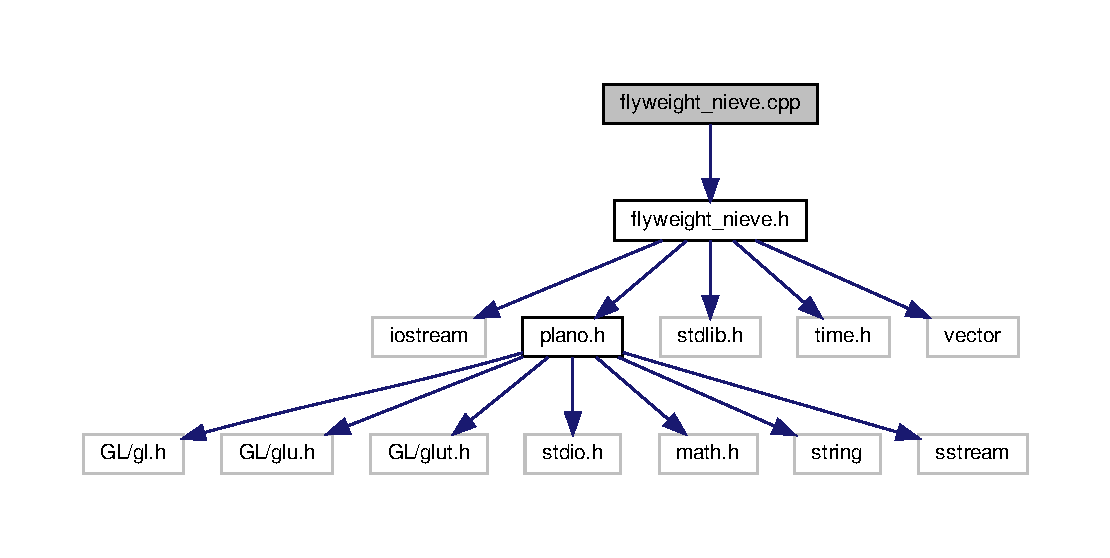
\includegraphics[width=350pt]{flyweight__nieve_8cpp__incl}
\end{center}
\end{figure}


\subsection{Descripción detallada}
implementacion de la clase paints para la creacion de paints en Glut Open\+GL 

\begin{DoxyAuthor}{Autor}
Walker Manrique 
\end{DoxyAuthor}
\begin{DoxyVersion}{Versión}
Revision 1.\+1 
\end{DoxyVersion}

\hypertarget{flyweight__nieve_8h}{}\section{Referencia del Archivo flyweight\+\_\+nieve.\+h}
\label{flyweight__nieve_8h}\index{flyweight\+\_\+nieve.\+h@{flyweight\+\_\+nieve.\+h}}


implementacion de la clase paints para la creacion de paints en Glut Open\+GL  


{\ttfamily \#include $<$iostream$>$}\newline
{\ttfamily \#include \char`\"{}plano.\+h\char`\"{}}\newline
{\ttfamily \#include $<$stdlib.\+h$>$}\newline
{\ttfamily \#include $<$time.\+h$>$}\newline
{\ttfamily \#include $<$vector$>$}\newline
Dependencia gráfica adjunta para flyweight\+\_\+nieve.\+h\+:
\nopagebreak
\begin{figure}[H]
\begin{center}
\leavevmode
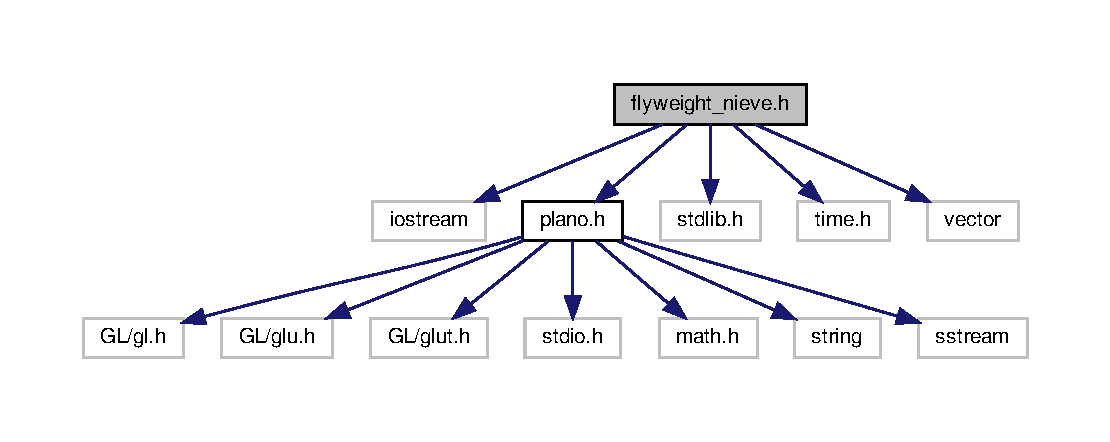
\includegraphics[width=350pt]{flyweight__nieve_8h__incl}
\end{center}
\end{figure}
Gráfico de los archivos que directa o indirectamente incluyen a este archivo\+:
\nopagebreak
\begin{figure}[H]
\begin{center}
\leavevmode
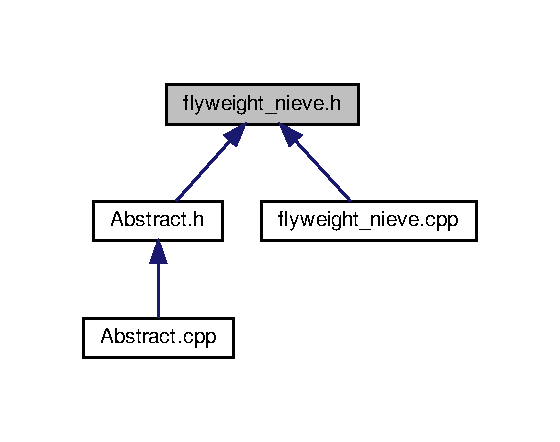
\includegraphics[width=269pt]{flyweight__nieve_8h__dep__incl}
\end{center}
\end{figure}
\subsection*{Clases}
\begin{DoxyCompactItemize}
\item 
class \hyperlink{classsnow__flyweight}{snow\+\_\+flyweight}
\begin{DoxyCompactList}\small\item\em La clase \hyperlink{classsnow__flyweight}{snow\+\_\+flyweight} es el singleton que dibuja la nieve.  Se instancia el dato miembro. \end{DoxyCompactList}\item 
class \hyperlink{classparticles}{particles}
\begin{DoxyCompactList}\small\item\em La clase particles es la calse que dibuja solo una particula.  Se instancia el dato miembro. \end{DoxyCompactList}\item 
class \hyperlink{classnieve}{nieve}
\begin{DoxyCompactList}\small\item\em La clase nieve es la clase que crea las particulas de nieve.  Se instancia el dato miembro. \end{DoxyCompactList}\end{DoxyCompactItemize}


\subsection{Descripción detallada}
implementacion de la clase paints para la creacion de paints en Glut Open\+GL 

\begin{DoxyAuthor}{Autor}
Walker Manrique 
\end{DoxyAuthor}
\begin{DoxyVersion}{Versión}
Revision 1.\+1 
\end{DoxyVersion}

\hypertarget{plano_8cpp}{}\section{Referencia del Archivo plano.\+cpp}
\label{plano_8cpp}\index{plano.\+cpp@{plano.\+cpp}}


implementacion de clase plano que permite hacer dibujos usando open\+GL.  


{\ttfamily \#include \char`\"{}plano.\+h\char`\"{}}\newline
Dependencia gráfica adjunta para plano.\+cpp\+:
% FIG 0


\subsection{Descripción detallada}
implementacion de clase plano que permite hacer dibujos usando open\+GL. 

\begin{DoxyAuthor}{Autor}
Walker Manrique 
\end{DoxyAuthor}
\begin{DoxyVersion}{Versión}
Revision 1.\+1 
\end{DoxyVersion}

\hypertarget{plano_8h}{}\section{Referencia del Archivo plano.\+h}
\label{plano_8h}\index{plano.\+h@{plano.\+h}}


implementacion de clase plano que permite hacer dibujos usando open\+GL.  


{\ttfamily \#include $<$G\+L/gl.\+h$>$}\newline
{\ttfamily \#include $<$G\+L/glu.\+h$>$}\newline
{\ttfamily \#include $<$G\+L/glut.\+h$>$}\newline
{\ttfamily \#include $<$stdio.\+h$>$}\newline
{\ttfamily \#include $<$math.\+h$>$}\newline
{\ttfamily \#include $<$string$>$}\newline
{\ttfamily \#include $<$sstream$>$}\newline
Dependencia gráfica adjunta para plano.\+h\+:
\nopagebreak
\begin{figure}[H]
\begin{center}
\leavevmode
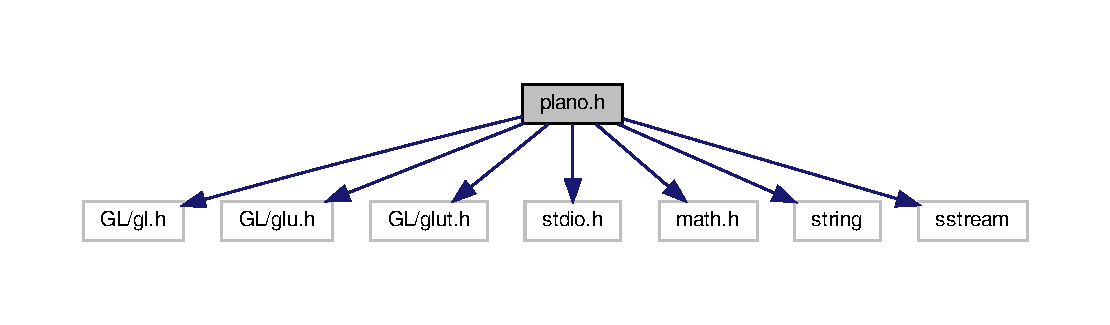
\includegraphics[width=350pt]{plano_8h__incl}
\end{center}
\end{figure}
Gráfico de los archivos que directa o indirectamente incluyen a este archivo\+:
\nopagebreak
\begin{figure}[H]
\begin{center}
\leavevmode
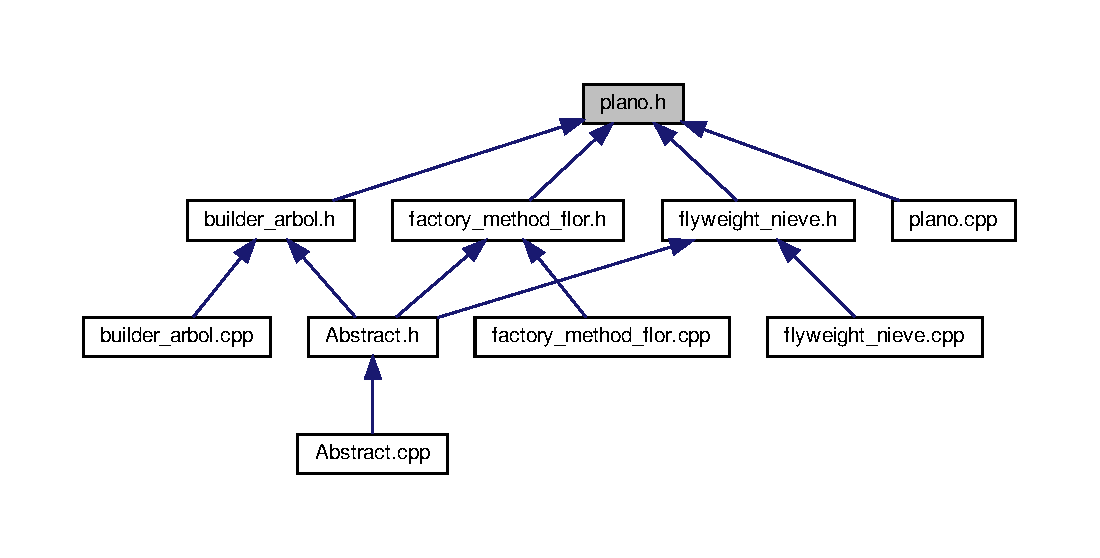
\includegraphics[width=350pt]{plano_8h__dep__incl}
\end{center}
\end{figure}
\subsection*{Clases}
\begin{DoxyCompactItemize}
\item 
struct \hyperlink{structcoordenada}{coordenada}
\item 
class \hyperlink{classplano}{plano}
\begin{DoxyCompactList}\small\item\em La clase plano tiene los elementos basicos para empezar a dibujar como se hace en la python turtle.  Definicion de la funciones usadas en la clase. \end{DoxyCompactList}\end{DoxyCompactItemize}
\subsection*{defines}
\begin{DoxyCompactItemize}
\item 
\mbox{\Hypertarget{plano_8h_a598a3330b3c21701223ee0ca14316eca}\label{plano_8h_a598a3330b3c21701223ee0ca14316eca}} 
\#define {\bfseries PI}~3.\+1415926535897932384626433832795
\end{DoxyCompactItemize}
\subsection*{typedefs}
\begin{DoxyCompactItemize}
\item 
\mbox{\Hypertarget{plano_8h_abce788b74b2513b814786f28fcdd11f7}\label{plano_8h_abce788b74b2513b814786f28fcdd11f7}} 
typedef double {\bfseries t\+\_\+coord}
\end{DoxyCompactItemize}


\subsection{Descripción detallada}
implementacion de clase plano que permite hacer dibujos usando open\+GL. 

\begin{DoxyAuthor}{Autor}
Walker Manrique 
\end{DoxyAuthor}
\begin{DoxyVersion}{Versión}
Revision 1.\+1 
\end{DoxyVersion}

%--- End generated contents ---

% Index
\backmatter
\newpage
\phantomsection
\clearemptydoublepage
\addcontentsline{toc}{chapter}{Índice}
\printindex

\end{document}
